\documentclass{article}
\usepackage{graphicx} % Required for inserting images
\usepackage[margin=2cm, top=3cm]{geometry} % margine superiore ridotto a 1 cm
\usepackage{listings}
\usepackage{subcaption}  % Pacchetto per sottodidascalie
\usepackage{float}       % Pacchetto per posizionamento rigido delle figure
\usepackage{xcolor} % Pacchetto per i colori
\usepackage{amsmath} % Pacchetto per simboli avanzati

\title{Machine Learning Esonero}
\author{Mattia Cosimi}
\date{December 2024}

\begin{document}

\maketitle

\section{Fondamenti di ML}
\subsection{Dati e Pattern}
I dati sono un ingrediente fondamentale del machine learning dove il comportamento degli algoritmi non è pre-programmato ma appreso dai dati stessi. Utilizzeremo spesso il termine \textbf{Pattern} per riferirci ai dati. La disciplina che studia il riconoscimento dei pattern prende il nome di \textbf{Pattern Recognition}.
\subsubsection{Tipi di Pattern}
\vspace{10pt}
\textbf{Numerici}: valori associati a caratteristiche misurabili o conteggi.\\
Sono rappresentabili naturalmente come vettori numerici nello spazio multidimensionale. L'estrazione di caratteristiche da segnali produce vettori numerici detti anche feature vectors. Es. Persona [altezza, circonferenza toracica, circonferenza fianchi, lunghezza del piede]
\\\\
\textbf{Categorici}: valori associati a caratteristiche qualitative e alla presenza/assenza di una caratteristica (yes/no value).
\\
Non sono mappabili in valori numerici. Es. Persona: [sesso, maggiorenne, colore occhi, gruppo sanguigno]. Solitamente vengono gestiti da sistemi a regole e alberi di classificazione. Molto utilizzati nell'ambito del \textbf{data mining}.
\\\\
\textbf{Sequenze}: pattern sequenziali con relazioni spaziali o temporali.\\
Ne sono un esempio, uno stream audio (sequenza di suoni) corrispondente alla pronuncia di una parola, una frase (sequenza di parole) in linguaggio naturale, l'andamento di un titolo di borsa (sequenza temporale del prezzo di chiusura). La posizione nella sequenza e le relazioni con predecessori e successori sono importanti
\\\\
\textbf{Altri dati strutturati}: output organizzati in strutture complesse quali alberi e grafi. Esempio nella traduzione di una frase in linguaggio naturale, l'output desiderato è l'insieme dei parse tree plausibili.
\subsubsection{Classificazione}
Assegna una \textbf{classe} a un pattern. Risulta necessario apprendere una funzione capace di eseguire il mapping dallo spazio dei pattern allo spazio delle classi. Si usa spesso anche il termine riconoscimento. Nel caso di 2 sole classi si usa il termine \textbf{binary classification}, con più di due classi \textbf{multi-class classification}.\\
Esempi nel problema di classificazione: spam detection, face recognition...
\\Una classe è un insieme di pattern aventi proprietà comuni. Il concetto di classe è semantico e dipende strettamente dall'applicazione, es. 21 classi per il riconoscimento di lettere dell'alfabeto, 2 classi per distinguere le lettere dell'alfabeto italiano da quello cirillico.
\subsubsection{Regressione}
Assegna un \textbf{valore continuo} a un pattern. Risulta utile per la predizione di valori continui. Risolvere un problema di regressione corrisponde ad apprendere una funzione approssimante delle coppie <<input, output>> date.\\
Es. stima dell'altezza di una persona in base al peso o stima prezzi vendita appartamenti nel mercato immobiliare.
\subsubsection{Clustering}
Individua \textbf{gruppi} (cluster) di pattern con caratteristiche simili. Le classi del problema non sono note (apprendimento non supervisionato) e i pattern non etichettati, la natura non supervisionata del problema lo rende più complesso della classificazione. I cluster individuati nell'apprendimento possono essere poi utilizzati come classi.\\
Es. Marketing: definizione di gruppi utenti in base ai consumi, Genetica: raggruppamento individui sulla base analogie DNA.
\subsubsection{Riduzione dimensionalità}
Riduce il numero di dimensioni dei pattern in input. Consiste nell'apprendimento di un mapping da $R^d$ a $R^k$ (con $k<d$). L'operazione comporta una perdita di informazione. L'obiettivo è conservare le informazioni importanti. 
\subsubsection{Representation Learning}
Il successo di molte applicazioni di machine learning dipende dall'efficacia di rappresentazione dei pattern in termini di features. La definizione di features ad-hoc per le diverse applicazioni prende il nome di \textbf{feature engineering}. Ad esempio per il riconoscimento di oggetti esistono numerosi descrittori di forma, colore e tessitura che possiamo utilizzare per convertire immagini in vettori numerici. Volendo si potrebbe apprendere anche da raw data e un esempio sono proprio le tecniche di \textbf{Deep Learning} (es. convolutional neural networks) che utilizzano in input raw data ed estraggono automaticamente da essi le feature necessarie per risolvere il problema d'interesse.

\subsubsection{Problemi di Computer Vision}
\begin{figure}[H] % Usa 'H' per forzare la posizione qui
    \centering % Centra l'immagine
    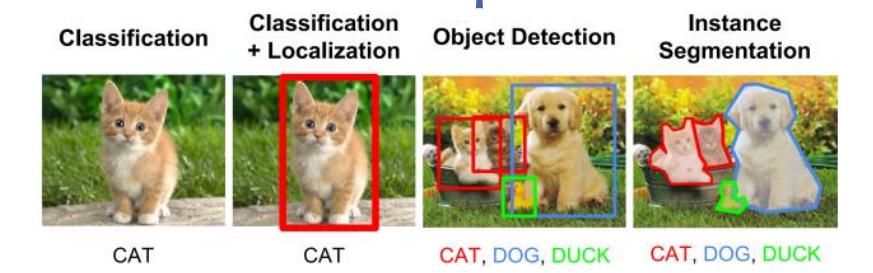
\includegraphics[width=11cm, height=3cm]{immagine_2024-12-10_121720256.png} % Percorso dell'immagine
    \caption{} % Didascalia per l'immagine
    \label{fig:immagine} % Etichetta per riferimento
\end{figure}
\noindent
\textbf{Classification}: determina la classe dell'oggetto. \textbf{Classification e Localization}: determina la classe dell'oggetto e la sua posizione nell'immagine. \textbf{Detection}: per ogni oggetto determina la classe e la posizione nell'immagine. \textbf{Segmentation}: al posto di una bounding box etichetta i singoli pixel dell'immagine a classi con indici delle classi.
\subsection{\textcolor{red} {Apprendimento}}
\subsubsection{Supervisionato (supervised)}
Sono note le classi dei pattern utilizzati per l'addestramento. Il training set è etichettato. Situazione tipica nella classificazione, regressione e in alcune tecniche di riduzione di dimensionalità.
\subsubsection{Non supervisionato (Unsupervised)}
Non sono note le classi dei pattern utilizzati per l'addestramento. Il training set non è etichettato. Situazione tipica nel clustering e nella maggior parte di tecniche di riduzione di dimensionalità.
\subsubsection{Semi-Supervizionato (Semi-Supervised)}
Il training set è etichettato parzialmente, la distribuzione dei pattern non etichettati può aiutare a ottimizzare la regola di classificazione.
\subsubsection{Batch}
L'addestramento è effettuato una sola volta su un training set dato. Una volta terminato il training, il sistema passa in $<<$Working mode$>>$
e non è in grado di apprendere uteriormente. 
\subsubsection{Incrementale}
A seguito dell'addestramento iniziale, sono possibili ulteriori sessioni di addestramento, es. sequenze di Batch, il rischio principale è il catastrofic forgetting ovvero il sistema dimentica quello che ha appreso in precedenza.
\subsubsection{Naturale}
Addestramento continuo (per tutta la vita), coesistenza di approccio supervisionato e non supervisionato
\subsubsection{Reinforcement Learning}
L'obiettivo è apprendere un comportamento ottimale a partire dalle esperienze passate. Un agente esegue \textbf{azioni} che modificano l'\textbf{ambiente}, provocando passaggi da uno \textbf{stato} all'altro. Quando l'agente ottiene risultati positivi riceve una ricompensa (\textbf{reward}) che però può essere temporalmente ritardata rispetto all'azione, o alla sequenza di azioni, che l'hanno determinata. Obiettivo è apprendere l'azione ottimale in ciascun stato, in modo da massimizzare la somma dei reward ottenuti nel lungo periodo.\\
Trova numerose applicazioni in \textbf{Robotica}, una sua estensione (deep) denominata \textbf{Deep Reinforcement Learning (DRL)} è alla base dei successi ottenuti da Google DeepMind
\section{\textcolor{red} {Parametri e Funzione Obiettivo}}
\subsection{Funzione obiettivo}
In genere, il comportamento di un algoritmo di Machine Learning è regolato da un set di parametri $\theta$. L'apprendimento consiste nel determinare il valore ottimo $\theta *$ di questi parametri. Dato un training set \textbf{Train} e un insieme di parametri, la \textbf{funzione obiettivo} $f(Train, \theta)$ può indicare:\\
L'\textbf{ottimalità} della soluzione (da massimizzare): $$\theta* = argmax_\theta f(Train, \theta)$$
Oppure l'errore o perdita (\textbf{loss-function}) da minimizzare.
$$\theta*= argmin_\theta f(Train, \theta)$$
$f(Train, \theta)$ può essere ottimizzata: \textbf{esplicitamente}, con metodi che operano a partire dalla sua definizione matematica. Es. si calcolano del derivate parziali di f rispetto ai parametri (gradiente), si eguaglia il gradiente a 0 (sistema di equazioni) e si risolve rispetto ai parametri. O \textbf{implicitamente}, utilizzando euristiche che modificano i parametri in modo coerente con f. Es. clustering con algoritmo k-means.
\subsection{\textcolor{red}{Iperparametri}}
Molti algoritmi richiedono di definire, prima dell'apprendimento vero e proprio, il valore dei cosiddetti iperparametri H.\\\\
Sono un esempio: il numero di neuroni di una rete neurale, il numero di vicini k in un classificatore k-NN, il grado di un polinomio utilizzato in una regressione, il tipo di loss function.\\\\
Si procede con un approccio a due livelli nel quale per ogni valore \textbf{ragionevole} degli iperparametri si esegue l'apprendimento, e al termine della procedura si scelgono gli iperparametri che hanno fornito \textbf{prestazioni migliori}.
\subsubsection{\textcolor{red} {Valutazione delle prestazioni}}
Una possibilità consiste nell'utilizzare direttamente la funzione obiettivo per quantificare le prestazioni. In genere però si preferisce una misura legata direttamente alla semantica del problema. \\
In un problema di \textbf{Classificazione} l'accuratezza di classificazione 
$[0...100\%]$ è la percentuale di pattern correttamente classificati. L'errore di classificazione è il complemento.
$$Accuratezza=\frac{pattern\ correttamente \ classificati}{pattern \ classificati}$$
$$Errore=100\%-Accuratezza$$
Attenzione ai problemi di classificazione con cardinalità classi molto sbilanciate: Es. in un problema di classificazione binaria, se una delle due
classi è rara, un classificatore "dummy" che non la predice
mai potrebbe raggiungere un’accuratezza di classificazione
vicina al 100\%. Meglio usare Precision/Recall in questo caso.
\\\\
Nei problemi di \textbf{Regressione}, si valuta in genere l' \textbf{RMSE (Root Mean Squared Error)} ovvero la radice della media dei quadrati degli scostamenti tra valore vero e valore predetto. 
$$RMSE= \sqrt{\frac{1}{N}\sum_{i=1}^{N}(pred_i-true_i)^2}$$
\subsubsection{Matrice di Confusione}
La matrice di confusione (confusion matrix) è molto utile nei problemi di \textbf{classificazione} (multiclasse) per capire come sono distribuiti gli errori. Nell'esempio un problema di classificazione digit (10 classi). \\
Sulle righe le classi \textbf{true} sulle colonne le classi predicted. Una cella (r,c) riporta la percentuale di casi in cui il sistema ha predetto di classe c un pattern di classe vera r. Idealmente la matrice dovrebbe essere diagonale. Valori elevati (fuori diagonale) indicano concentrazioni di errori.
\begin{figure}[H] % Usa 'H' per forzare la posizione qui
    \centering % Centra l'immagine
    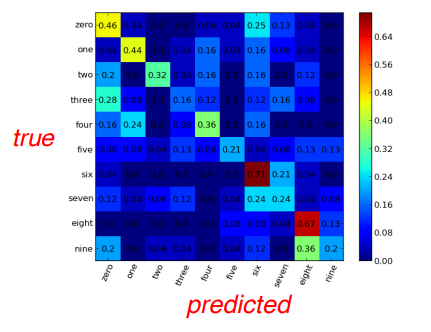
\includegraphics[width=6cm, height=5cm]{immagine_2024-12-10_162451052.png} % Percorso dell'immagine
    \caption{} % Didascalia per l'immagine
    \label{fig:immagine} % Etichetta per riferimento
\end{figure}
\subsubsection{Problemi Closed e Open Set}
Nel caso \textbf{più semplice} si assume che il pattern da classificare appartenga a una delle classi note (\textbf{closed set}). Es. classificare le persone in \{uomini, donne\}. In molti casi reali invece i pattern da classificare possono appartenere a una delle classi note o a nessuna di queste (\textbf{open set}). Es. classificare tutta la frutta in \{mele, pere, banane\}. Per fare questo ci sono due soluzioni principali: Si aggiunge alle classi un'ulteriore classe fittizia "il resto del mondo" e si aggiungono al training set i cosiddetti "esempi negativi". Si consente al sistema di non assegnare il pattern. A tal fine si definisce una soglia e si assegna il pattern alla classe più probabile solo quando la probabilità è superiore alla soglia.
\subsubsection{\textcolor{red} {Classificazione binaria}}
Consideriamo un problema di classificazione binario, dove le due classi corrispondono a esempi \textbf{Positivi} (vera classe) e \textbf{Negativi} (classe fittizia resto del mondo). Es. face detection. Positivi: tutte le porzioni di immagine (finestre) in cui appaiono volti. Negativi: finestre (scelte a caso) in cui non compaiono volti. Analogamente possiamo considerare solo la classe positivi e un sistema (con soglia) in grado di calcolare la probabilità p di appartenenza di un pattern alla classe. Sia t il valore della soglia, allora il pattern viene classificato come positivo se $ p > t$, come negativo in caso contrario. \\
Dato un classificatore binario e $T=P+N$ pattern da classificare (P positivi e N negativi), il risultato di ciascuno dei tentativi di classificazione può essere: \textbf{True Positive (TP)}: un pattern positivo è stato correttamente assegnato ai positivi, \textbf{True Negative (TN)}: un pattern negativo è stato correttamente assegnato ai negativi, \textbf{False Positive (FP)}: un pattern negativo è stato erroneamente assegnato ai positivi. Detto anche errore di Tipo I o False. \textbf{False Negative (FN)}: un pattern positivo è stato erroneamente assegnato ai negativi. Detto anche errore di Tipo II o Miss.\\
Passando da errori a frequenze/probabilità:
$$TPR \ (True \ Positive \ Rate) = \frac{TP}{P}$$
$$TNR \ (True \ Negative \ Rate) = \frac{TN}{N}$$
$$FPR \ (False \ Positive \ Rate) = \frac{FP}{N}$$
$$FNR \ (False \ Negative \ Rate) = \frac{FN}{P}$$
Con questa notazione l'accuratezza di classificazione può essere scritta come: $$Accuracy=\frac{TP+TN}{T=P+N}$$
\subsubsection{\textcolor{red} {Sistemi con soglia (DET e ROC)}}
Nei sistemi con soglia false positive rate e false negative rate sono \textbf{funzione} della soglia t. Soglie restrittive (elevate) riducono i false positive a discapito dei false negative; viceversa soglie tolleranti (basse) riducono i false negative a discapito dei false positive.
\begin{figure}[H] % Usa 'H' per forzare la posizione qui
    \centering % Centra l'immagine
    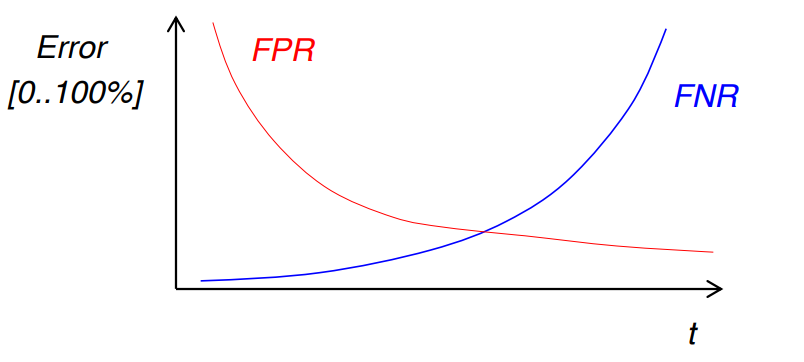
\includegraphics[width=6cm, height=4cm]{Screenshot 2024-12-10 175415.png} % Percorso dell'immagine
    \caption{} % Didascalia per l'immagine
    \label{fig:immagine} % Etichetta per riferimento
\end{figure}
\vspace{200pt}
\noindent
Le due curve possono essere "condensate" in una curva \textbf{DET (Detection Error Tradeoff)} che nasconde la soglia. Piuttosto usata è anche la rappresentazione \textbf{ROC (Receiver Operating Characteristic)} che in ordinata riporta True positive invece di False negative (ROC è ribaltata verticalmente rispetto a DET).
\begin{figure}[H] % Usa 'H' per forzare la posizione qui
    \centering % Centra l'immagine
    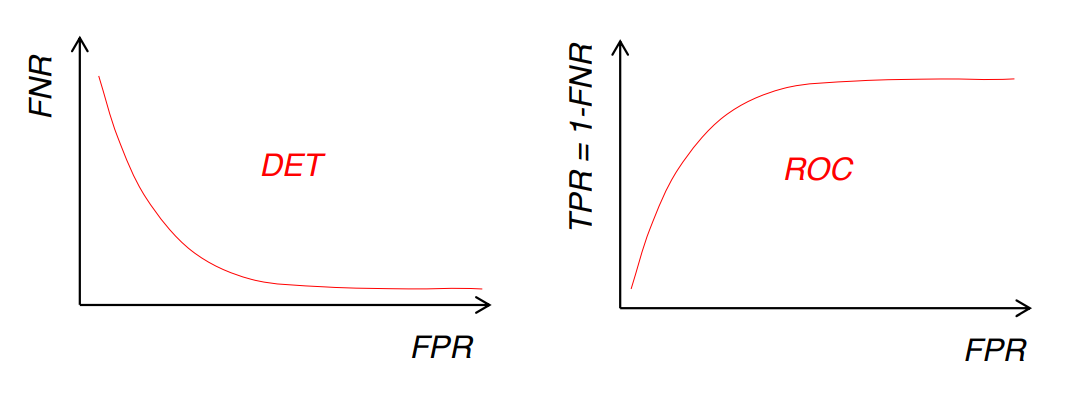
\includegraphics[width=10cm, height=4cm]{immagine_2024-12-10_180105841.png} % Percorso dell'immagine
    \caption{} % Didascalia per l'immagine
    \label{fig:immagine} % Etichetta per riferimento
\end{figure}
Quale dei due sistemi (rosso, blu) è migliore dell'altro?
\begin{figure}[H] % 'h' per indicare di posizionare la figura qui
    \centering % Centra l'intera figura
    % Immagine di sinistra
    \begin{subfigure}[t]{0.35\textwidth} % Sottotitolo di dimensione 45% della larghezza
        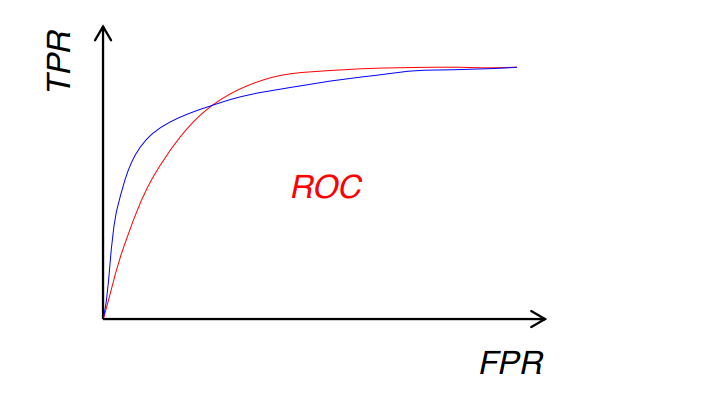
\includegraphics[width=\linewidth]{immagine_2024-12-10_180535374.png} % Percorso dell'immagine
       % \caption{Arrivo in precedenza dei processi più piccoli} % Didascalia per la prima immagine
        \label{fig:sinistra} % Etichetta per riferimento
    \end{subfigure}
    \hspace{0.05\textwidth} % Spazio orizzontale tra le immagini
    % Immagine di destra
    \begin{subfigure}[t]{0.35\textwidth} % Sottotitolo di dimensione 45% della larghezza
        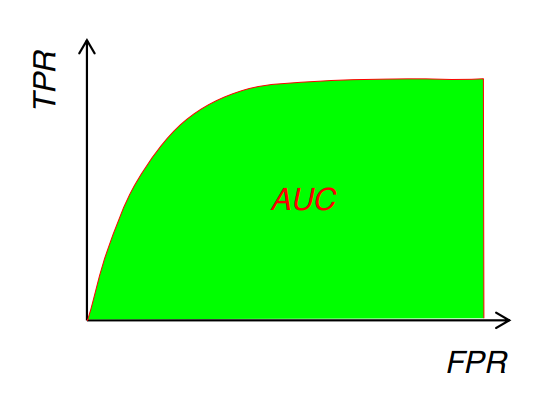
\includegraphics[width=\linewidth]{immagine_2024-12-10_180808866.png} % Percorso dell'immagine
       % \caption{Arrivo in precedenza del processo più grande} % Didascalia per la seconda immagine
        \label{fig:destra} % Etichetta per riferimento
    \end{subfigure}
   % \caption{SJF/Shortest Job First} % Didascalia generale per la figura
    \label{fig:due_immagini} % Etichetta generale per riferimento
\end{figure}
\noindent
Il sistema migliore è quello la cui curve è più "alta", ma in questo caso le curve si intersecano ... e l'ottimalità dipende dal punto di lavoro desiderato. Un confronto può essere fatto "mediando" sui diversi punti di lavoro del sistema. L'\textbf{area sotto la curva ROC (AUC)} è uno scalare in [0,1] che caratterizza la prestazione media (maggiore è, meglio è). Può essere calcolata come integrale numerico.\\
Un tipico esempio di sistemi con soglia sono i \textbf{sistemi biometrici} di verifica di identità: Questa immagine dell'iride è del soggetto Q?\\
False positive e False negative in questo caso prendono il nome di \textbf{False Match} e \textbf{False Non-Match}. Nel caso open set multi-classe, nella biometria si parla anche di \textbf{identificazione} distinguendola dalla verifica di identità e si definiscono FPIR (False Positive Identification Rate) e FNIR (False Negative Identification Rate).
\subsubsection{\textcolor{red} {Precision e Recall}}
Notazione molto usata in Information Retrieval e in generale nelle applicazioni di detection. \textbf{Precision} indica quanto è accurato il sistema. (quanti True sono veri su quanti True ha dato)\\
Che percentuale di documenti selezionati è pertinente?$$Precision = \frac{TP}{TP+FP}$$ \textbf{Recall} quanto è selettivo. (Quanti True su quelli che sono tutti i true possibili True positive e False Negative)\\
Di tutti i documenti pertinenti quanti ne sono stati selezionati?
$$Recall=\frac{TP}{TP+FN}=\frac{TP}{P}=TPR$$
Un'altra rappresentazione grafica utile per comprendere Precision e Recall è la matrice di confusione 2x2 che evidenzia \textbf{TN, TP, FP, FN}: Il classificatore (binario) dell'esempio sotto ha come classe positiva il digit 5 e come classe negativa tutti gli altri digit.
\begin{figure}[H] % Usa 'H' per forzare la posizione qui
    \centering % Centra l'immagine
    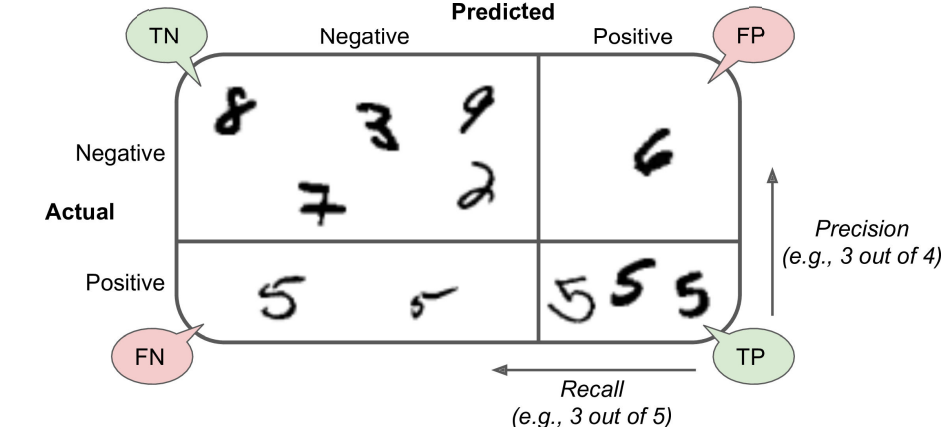
\includegraphics[width=10cm, height=4cm]{immagine_2024-12-10_182941080.png} % Percorso dell'immagine
    \caption{} % Didascalia per l'immagine
    \label{fig:immagine} % Etichetta per riferimento
\end{figure}
\begin{figure}[H] % Usa 'H' per forzare la posizione qui
    \centering % Centra l'immagine
    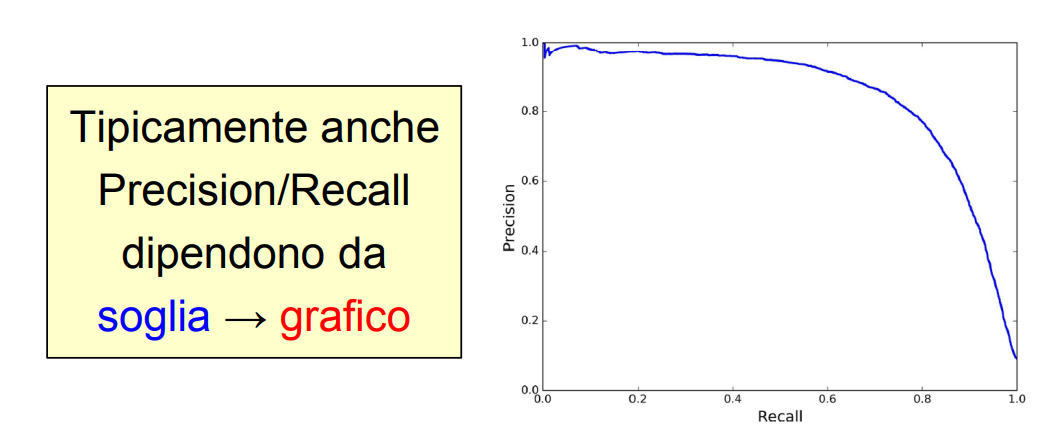
\includegraphics[width=10cm, height=4cm]{immagine_2024-12-10_183310541.png} % Percorso dell'immagine
    \caption{} % Didascalia per l'immagine
    \label{fig:immagine} % Etichetta per riferimento
\end{figure}
\noindent
Ogni punto della curva corrisponde a una soglia diversa e la sua posizione corrisponde alla Precision e alla Recall che si ottengono quando si sceglie quella soglia.
\subsubsection{Sensitivity e Specificity}
In diagnostica medica si usano i termini Sensitivity e Specificity per caratterizzare la bontà di un test (es. tampone Covid-19). Sensitivity=Recall (Tra tutti i sottoposti al test quanti infetti sono correttamente identificati come tali?)\\ 
Specificity indica quanto è accurato il sistema. (Che percentuale di non-infetti sottoposti al test sono stati dichiarati sani?)
\subsubsection{Object Detection: AP e mAP}
\textbf{Detection}: per ogni oggetto presente determina la probabilità di appartenenza alla classe più probabile e la corrispondente bounding box (una certa area). Ci possono essere diversi tipi di errori tra cui: oggetto non trovato, classe errata, bounding box sbagliata o imprecisa. Per rendere i sistemi confrontabili, si usa:\\
\textbf{Average Precision (AP)}: è una sorta di AUC calcolata su grafico Recall/Precision per oggetti di una singola classe su tutto il database
\textbf{medium Average Precision (mAP)}: è la media di AP su tutte le classi.\\
Per calcolare TP, FP si considera prediction corretta quando la classe è giusta e la Intersection over Union (IoU) delle due bounding box (rilevata e vera) è maggiore di un valore dato.
\section{\textcolor{red}{Training, Validation, Test, Domanda: Come configurare un Data Set}}
Il \textbf{Training} Set (Train) è l'insieme di pattern su cui addestrare il sistema, trovando il valore ottimo per i parametri $\theta$. Serve a trovare i parametri del sistema.\\\\
Il \textbf{Validation} Set (Valid) è l'insieme di pattern su cui tarare gli iperparametri H (ciclo esterno). Individuo gli iperparametri
Il \textbf{Test} Set (Test) è l'insieme di pattern su cui valutare le prestazioni finali del sistema. Sempre forte è la tentazione di tarare gli iperparametri sul test set (overfitting), va evitato.
\subsubsection{\textcolor{red} {K-fold Cross-Validation}}
Una scelta più robusta degli \textbf{iperparametri} si ottiene con la procedura di k-fold Cross-Validation. Nell'ipotesti 15 000 \textbf{pattern} totali e \textbf{k}=5: 5000 pattern sono \textbf{scorporati a priori} per il Test, i 10 000 pattern rimanenti sono suddivisi in 5 gruppi (fold) da 2000 pattern ciascuno. \\
Per ogni combinazione di \textbf{iperparametri $H_i$} che si vuole valutare:\\
Si esegue 5 volte il training scegliendo uno dei fold come Valid e i 4 rimanenti come Train\\
Si calcola l'accuratezza \textbf{$avg\_acc_i$} come media/mediana delle 5 accuratezze sui rispettivi Valid,\\
Si sceglie la combinazione di iperparametri con migliore \textbf{$avg\_acc$}\\
Scelti gli iperparametri ottimali \textbf{si riaddestra il modello su tutto il training set} (5 fold) e, solo a questo punto, si verificano le prestazioni sul \textbf{test set}.
\subsubsection{Partizionare i Dati}
Partizionare i dati in \textbf{Training, Validation e Test}, richiede in genere di generare (random) gli indici degli elementi da assegnare ai diversi insiemi per poi procedere alla suddivisione facendo attenzione a dividere nello stesso modo anche le etichette (in classificazione) o valori target (nella regressione). La funzione \textbf{train\_test\_split} di \textbf{Scikit Learn} automatizza, questa fase, a partire dalle proporzioni specificate in input, fornendo anche supporto per \textbf{shuffling} (ordinamento casuale dei pattern) e \textbf{stratification} (selezione bilanciata rispetto a certe categorie o insiemi di valori).\\
Relativamente a \textbf{Cross Validation Scikit Learn} mette a disposizione la funzione \textbf{$cross_val_score$} che a partire da un unico training set e il numero k di fold, valuta k volte il sistema e ritorna un array di K score.
\subsubsection{Selezione Automatica Iperparametri}
La ricerca di valori ottimali per gli iperparametri può essere lunga e noiosa. Automatizzare quando possibile:\\
\textbf{Grid Search}: per ogni iperparametro si definisce un insieme di valori da provare. Il sistema è valutato su tutte le combinazioni di valori di tutti gli iperparametri. \\
\textbf{Random Search}: sorteggia casualmente valori di iperparametri dai range/distribuzioni specificati/e, eseguendo un numero prefissato di iterazioni.
\subsubsection{Convergenza}
Il primo obiettivo da perseguire durante l'addestramento è la \textbf{convergenza} sul Train set. Consideriamo un classificatore il cui addestramento prevede un processo \textbf{iterativo}. Si ha convergenza quando: La \textbf{Loss} (output della loss function) ha andamento \textbf{decrescente}, l'\textbf{accuratezza} ha un andamento \textbf{crescente}.
\begin{figure}[H] % Usa 'H' per forzare la posizione qui
    \centering % Centra l'immagine
    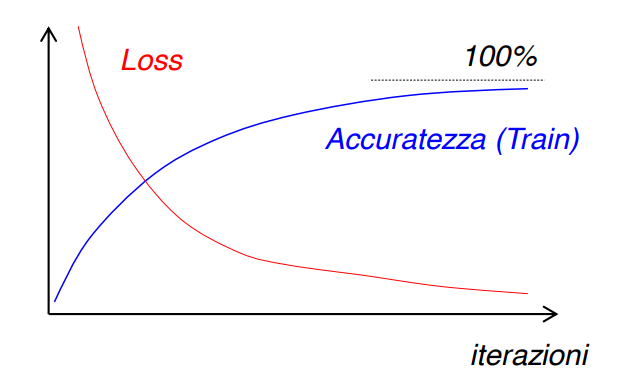
\includegraphics[width=5cm, height=2cm]{immagine_2024-12-12_122523116.png} % Percorso dell'immagine
    \caption{} % Didascalia per l'immagine
    \label{fig:immagine} % Etichetta per riferimento
\end{figure}
\noindent
Se la \textbf{loss non decresce} (o \textbf{oscilla} significativamente) il sistema non converge: il metodo di ottimizzazione non è efficace, gli iperparametri sono fuori range, il learning rate è inadeguato, ci sono errori di implementazione, ecc... \\
Se la \textbf{loss decresce ma l'accuratezza non crescce} probabilmente è stata scelta una loss-function errata.\\
Se l'\textbf{accuratezza non si avvicina al $100\%$ sul Train}, i gradi di libertà del classificatore non sono sufficienti per gestire la complessità del problema.
\subsubsection{Generalizzazione e Overfitting}
Per \textbf{generalizzazione} intendiamo la capacità di \textbf{trasferire} l'elevata accuratezza raggiunta su Train a Valid. Se i gradi di libertà del classificatore sono eccessivi, si raggiunge elevata accuratezza su Train, ma non su Valid (scarsa generalizzazione). In questo caso si parla di \textbf{overfitting} di Train. Questa situazione si verifica molto facilmente quando Train è di piccole dimensioni. Nei processi di addestramento iterativo, tipicamente dopo un certo numero di iterazioni l'accuratezza su Valid non aumenta più (e può iniziare a decrescere) a causa dell'overfitting. Monitorando l'andamento si può \textbf{arrestare l'addestramento} nel punto ideale (\textbf{early stopping}).
\subsubsection{Controllare l'Overfitting per massimizzare la Generalizzazione}
I gradi di libertà del classificatore non devono essere eccessivi, ma adeguati rispetto alla complessità del problema. Buona norma partire \textbf{con pochi gradi di libertà} (controllabili attraverso iperparametri) e \textbf{via via aumentarli} monitorando accuratezza su Train e Valid. I gradi di libertà influenzano la \textbf{regolarità} della soluzione appresa. La regolarità della soluzione può essere talvolta controllata aggiungendo un \textbf{fattore regolarizzante} alla loss-function che penalizza soluzioni irregolari. Es. in una rete neurale si possono favorire soluzioni prive di pesi con valori elevati (\textbf{$L_2$ regularization}), oppure solo una parte dei pesi sono diversi da 0 (\textbf{$L_1$ regularitazion $->$ sparsity})
\subsubsection{In pratica}
Non utilizzate approcci di Machine Learning per problemi sui quali \textbf{non avete a disposizione sufficienti esempi} per il Training e il Test. Ci sono servizi che etichettano e collezionano dati al posto nostro. I pattern da collezionare devono essere \textbf{rappresentativi} del problema che vogliamo risolvere e vanno distribuiti adeguatamente. \textbf{Automatizzare con le librerie} le procedure di valutazione delle prestazioni. Scrivere \textbf{codice} strutturato ordinato, eseguite debug incrementale e unit testing.

\section{Regressione}
\subsection{Introduzione}
I modelli a regressione vengono utilizzati per prevedere variabili target su \textbf{scala continua}, il che li rende interessanti per risolvere molte questioni in ambito scientifico e anche industriale, come ad esempio: trovare relazioni fra variabili, valutare tendenze, effettuare previsioni. L'obiettivo di un modello a Regressione Lineare Semplice (univariata) consiste nell'individuare le relazioni esistenti tra un'unica caratteristica (la variabile descrittiva x) e una risposta continua (variabile target y).
\subsubsection{Esempio (previsione del prezzo di un andamento)}
Consideriamo il caso della previsione del prezzo di un appartamento (variabile target y) data la sua metratura (variabile descrittiva x). Tipicamente in casi come questo abbiamo a disposizione un certo numero di esempi (osservazioni), costituiti da appartamenti già venduti per ciascuno dei quali abbiamo a disposizione l'area in mq o in sq.ft. (x) e il prezzo pagato per l'acquisto (y). Ciascuna delle suddette osservazioni può essere rappresentata da un punto in un piano cartesiano x-y.
\begin{figure}[H] % Usa 'H' per forzare la posizione qui
    \centering % Centra l'immagine
    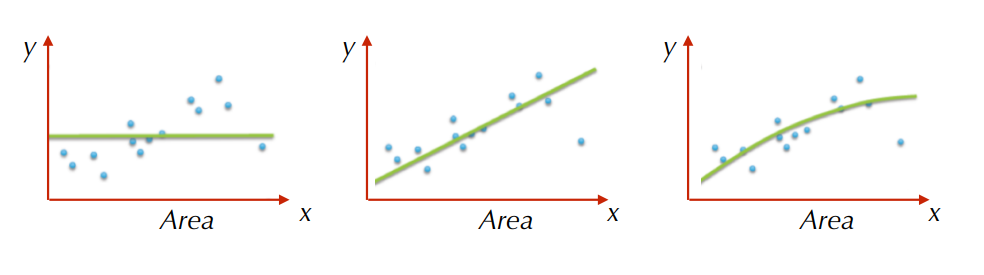
\includegraphics[width=10cm, height=3cm]{Screenshot 2024-12-11 141849.png} % Percorso dell'immagine
    \caption{} % Didascalia per l'immagine
    \label{fig:immagine} % Etichetta per riferimento
\end{figure}
\noindent
Il problema da risolvere è il seguente: scegliere lo spazio delle ipotesi \textcolor{green}{H} e la funzione \textcolor{green}{f(}\textcolor{red}{x}\textcolor{green}{)} (ipotesi) che approssima meglio le osservazioni disponibili di una funzione sconosciuta, da utilizzare per prevedere i prezzi di altri appartamenti.
\subsection{Simple Linear Regression Model}
In figura è rappresentato un modello lineare per \textcolor{green}{f(}\textcolor{red}{x}\textcolor{green}{)}, dove \textbf{$w_0$} rappresenta l'intercetta (punto in cui una retta o una curva incontra uno degli assi cartesiani) e il peso \textbf{$w_1$} rappresenta la pendenza della retta. Si noti l'offset verticale che costituisce l'errore che in genere esiste tra la previsione e il valore effettivo. Abbiamo dunque, il valore vero e quello previsto per un certo valore dell'ascissa.
\begin{figure}[H] % Usa 'H' per forzare la posizione qui
    \centering % Centra l'immagine
    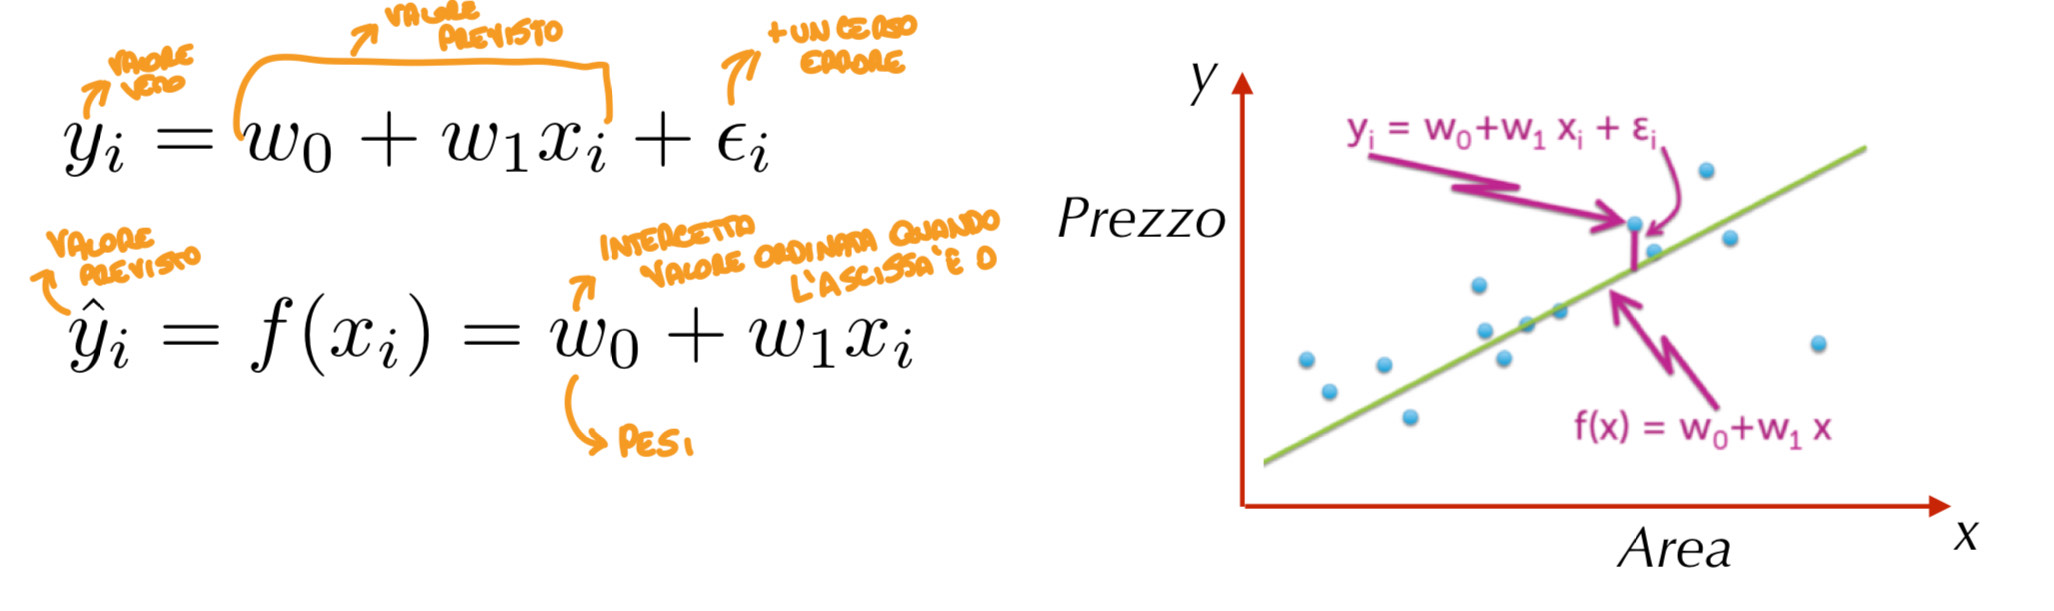
\includegraphics[width=11cm, height=4cm]{IMG_0837.jpeg} % Percorso dell'immagine
    \caption{} % Didascalia per l'immagine
    \label{fig:immagine} % Etichetta per riferimento
\end{figure}
\noindent
Una volta definito tale modello, ossia la forma della funzione \textcolor{green}{f(}\textcolor{red}{x}\textcolor{green}{)}, occorre determinare i due pesi incogniti, ossia l'intercetta e la pendenza, che definiscano la \textcolor{green}{f(}\textcolor{red}{x}\textcolor{green}{)} "migliore" secondo un certo criterio. Un criterio possibile è quello di minimizzare gli errori che si hanno sulle osservazioni.
\subsubsection{Residual Sum of Squares (RSS)}
Una delle funzioni utilizzate a tal fine, che deve essere per l'appunto minimizzata, è la \textbf{Residual Sum of Squares (RSS)}, definita come segue, a partire da N osservazioni disponibili:
\begin{figure}[H] % Usa 'H' per forzare la posizione qui
    \centering % Centra l'immagine
    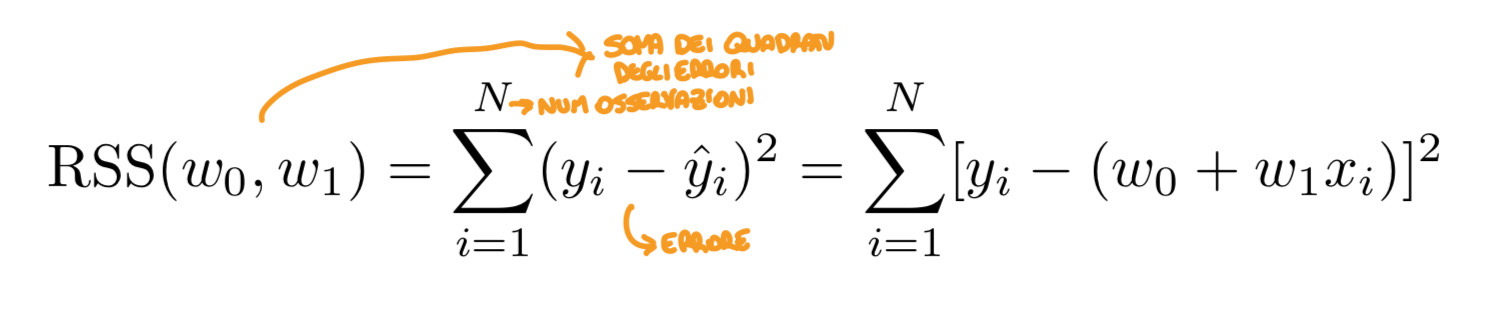
\includegraphics[width=13cm, height=3cm]{IMG_0838.jpeg} % Percorso dell'immagine
    \caption{} % Didascalia per l'immagine
    \label{fig:immagine} % Etichetta per riferimento
\end{figure}
\noindent
Il problema di addestrare il nostro modello è dunque quello di trovare i valori dei due pesi \( \hat{W_0} \) e \( \hat{W_1} \) che minimizzano la funzione \textbf{RSS}. In sintesi, il processo di apprendimento è formulato come una ricerca di ottimizzazione (ricerca del minimo) nello \textbf{spazio dei pesi}. A tal fine possiamo calcolare e avvalerci del \textbf{gradiente} della "misura d'errore" \textbf{RSS} definita in precedenza. Si può dimostrare che la \textbf{RSS} è una funzione convessa. Per funzioni convesse, quando il gradiente è uguale a zero si ha un minimo globale.
\begin{figure}[H] % Usa 'H' per forzare la posizione qui
    \centering % Centra l'immagine
    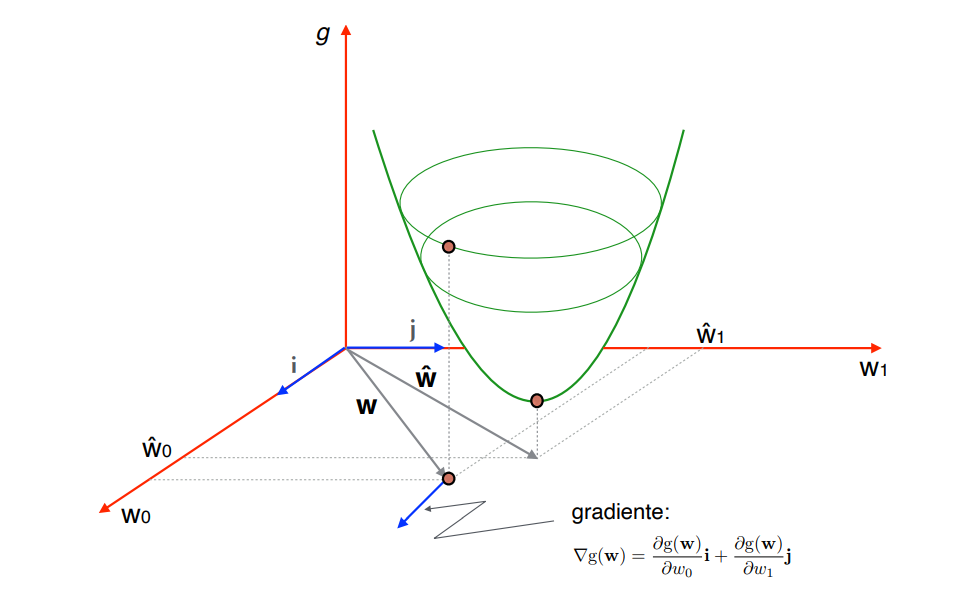
\includegraphics[width=11cm, height=7cm]{Screenshot 2024-12-11 160544.png} % Percorso dell'immagine
    \caption{} % Didascalia per l'immagine
    \label{fig:immagine} % Etichetta per riferimento
\end{figure}
\noindent
Quindi, per ottimizzare mi sposto verso il gradiente, per minimizzare mi sposto verso il lato opposto.
\subsubsection{Il processo di Training}
\begin{figure}[H] % Usa 'H' per forzare la posizione qui
    \centering % Centra l'immagine
    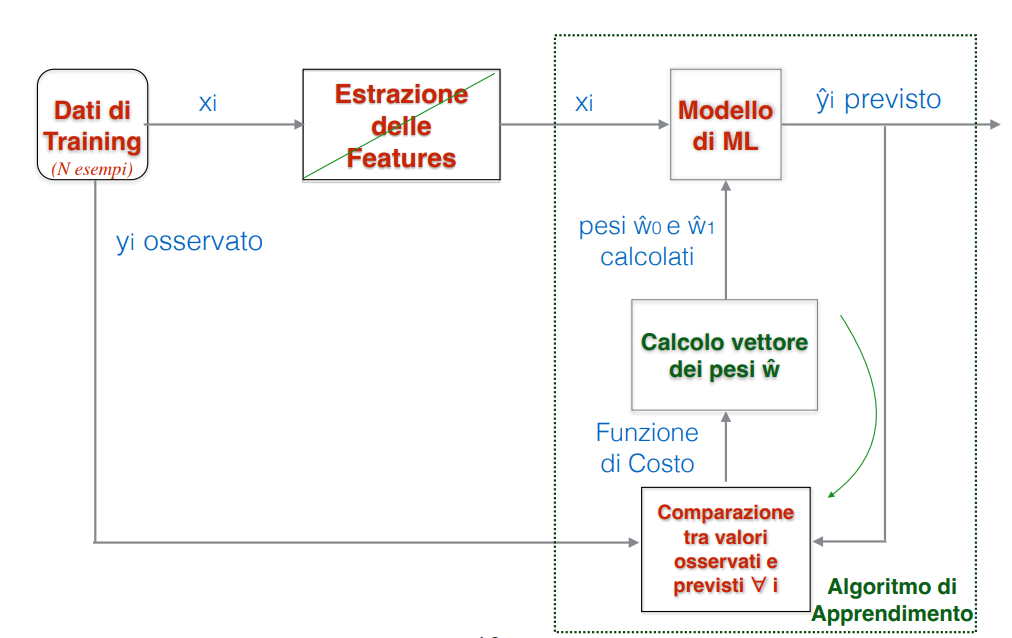
\includegraphics[width=11cm, height=7cm]{Screenshot 2024-12-11 164100.png} % Percorso dell'immagine
    \caption{} % Didascalia per l'immagine
    \label{fig:immagine} % Etichetta per riferimento
\end{figure}
\noindent
\textbf{Dati di training}: insieme di esempi ($x_i$, $y_i$) relativi a casi conosciuti (i punti nel piano x-y), da utilizzare per calcolare la funzione di costo RSS.\\
\textbf{Estrazione di features}: in questo caso tale funzione è inattiva, nel senso che riproduce in uscita il suo ingresso $x_i$.\\
\textbf{Modello di ML}: ipotesi f scelta, istanziata con i valori dei pesi più opportuni.\\
\textbf{Comparazione tra dati osservati e dati previsti}: per ogni esempio abbiamo il valore vero $y_i$ e il valore previsto \( \hat{y_i} \), da utilizzare per il calcolo della funzione RSS.\\
\textbf{Algoritmo di Apprendimento}: algoritmo che calcola i pesi che minimizzano la funzione di costo RSS, da utilizzare per definire il modello di ML.
\subsubsection{Gradiente della funzione RSS}
Il gradiente della funzione RSS:
\begin{figure}[H] % Usa 'H' per forzare la posizione qui
    \centering % Centra l'immagine
    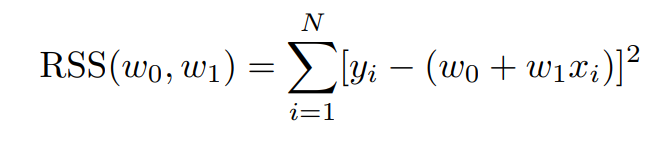
\includegraphics[width=11cm, height=2cm]{image.png} % Percorso dell'immagine
    \caption{} % Didascalia per l'immagine
    \label{fig:immagine} % Etichetta per riferimento
\end{figure}
\noindent
è definito come segue:
\begin{figure}[H] % Usa 'H' per forzare la posizione qui
    \centering % Centra l'immagine
    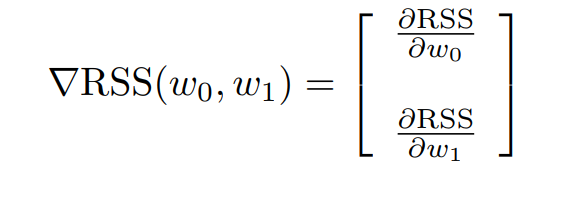
\includegraphics[width=7cm, height=2cm]{immagine_2024-12-11_163442154.png} % Percorso dell'immagine
    \caption{} % Didascalia per l'immagine
    \label{fig:immagine} % Etichetta per riferimento
\end{figure}
\begin{figure}[H] % Usa 'H' per forzare la posizione qui
    \centering % Centra l'immagine
    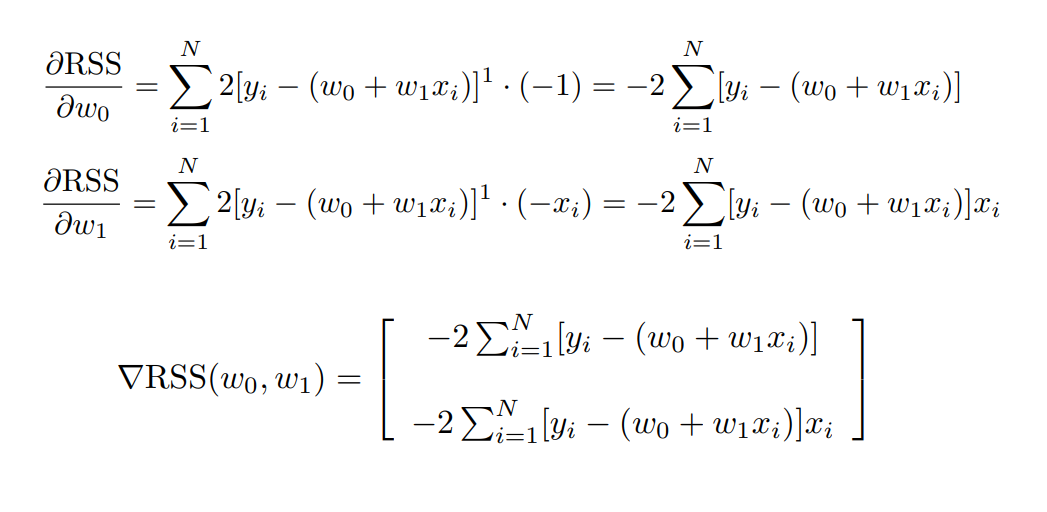
\includegraphics[width=11cm, height=6cm]{Screenshot 2024-12-11 163618.png} % Percorso dell'immagine
    \caption{} % Didascalia per l'immagine
    \label{fig:immagine} % Etichetta per riferimento
\end{figure}
\noindent
Una volta calcolato il gradiente della funzione \textbf{RSS}, ci sono due possibili approcci per minimizzare la funzione di costo: \textbf{"Forma chiusa"}, si eguaglia il gradiente a 0 (ossia al vettore nullo) e si risolvono le equazioni (non sempre è possibile o conveniente dal punto di vista computazionale). Algoritmo di Discesa del Gradiente (Hill climbing al contrario) (\textbf{Gradient Descent}) (richiede la definizione del criterio di convergenza e dello "step size"). Si parte da un punto dello spazio dei pesi, l'algoritmo si ferma quando arriva a un punto sufficientemente vicino al minimo assoluto.
\subsubsection{Forma Chiusa}
\begin{figure}[H] % 'h' per indicare di posizionare la figura qui
    \centering % Centra l'intera figura
    % Immagine di sinistra
    \begin{subfigure}[t]{0.45\textwidth} % Sottotitolo di dimensione 45% della larghezza
        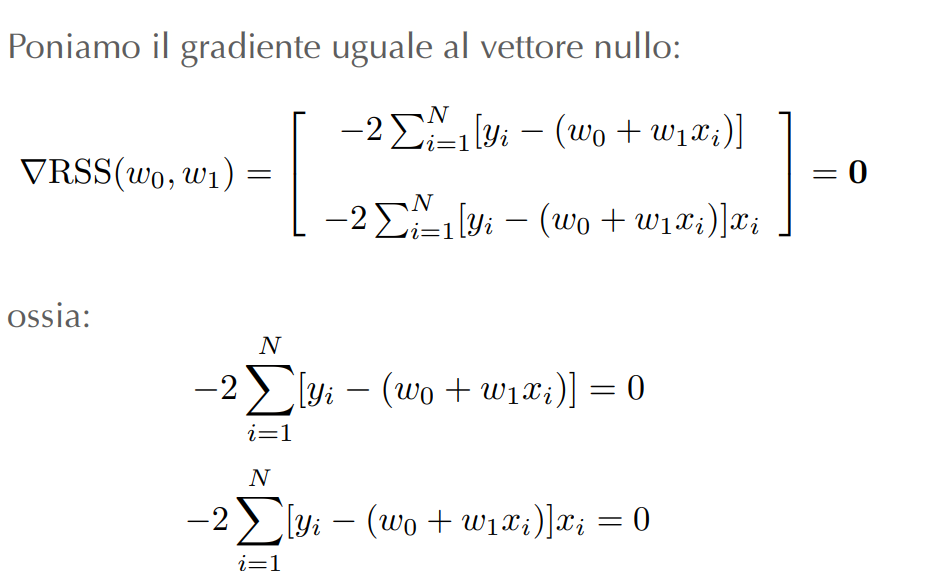
\includegraphics[width=\linewidth]{Screenshot 2024-12-11 165047.png} % Percorso dell'immagine
       % \caption{Arrivo in precedenza dei processi più piccoli} % Didascalia per la prima immagine
        \label{fig:sinistra} % Etichetta per riferimento
    \end{subfigure}
    \hspace{0.05\textwidth} % Spazio orizzontale tra le immagini
    % Immagine di destra
    \begin{subfigure}[t]{0.45\textwidth} % Sottotitolo di dimensione 45% della larghezza
        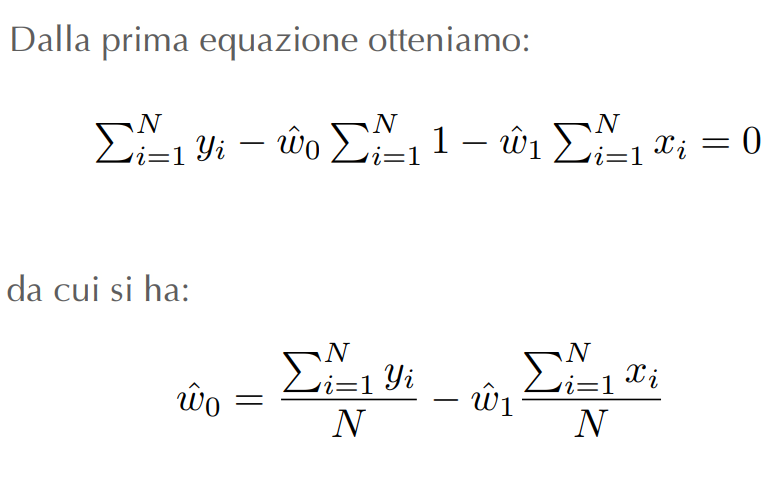
\includegraphics[width=\linewidth]{Screenshot 2024-12-11 165056.png} % Percorso dell'immagine
       % \caption{Arrivo in precedenza del processo più grande} % Didascalia per la seconda immagine
        \label{fig:destra} % Etichetta per riferimento
    \end{subfigure}
   % \caption{SJF/Shortest Job First} % Didascalia generale per la figura
    \label{fig:due_immagini} % Etichetta generale per riferimento
\end{figure}
\begin{figure}[H] % 'h' per indicare di posizionare la figura qui
    \centering % Centra l'intera figura
    % Immagine di sinistra
    \begin{subfigure}[t]{0.45\textwidth} % Sottotitolo di dimensione 45% della larghezza
        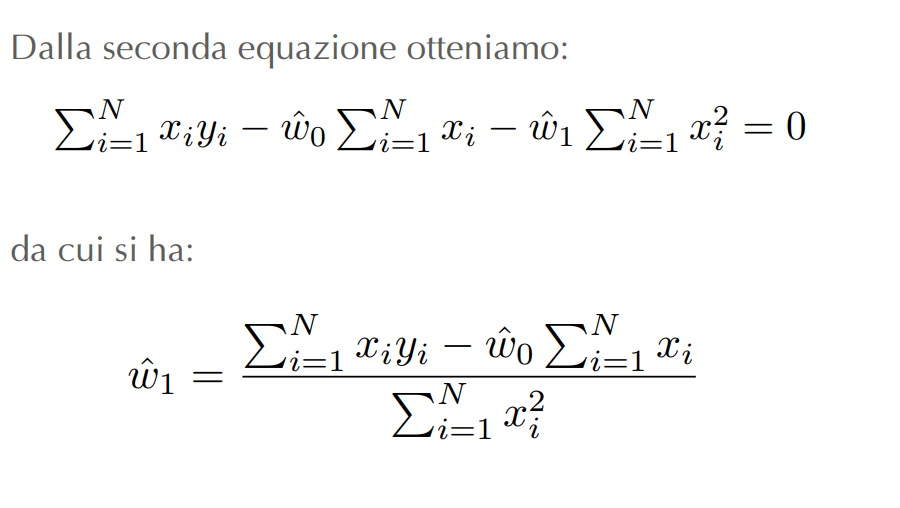
\includegraphics[width=\linewidth]{Screenshot 2024-12-11 165106.png} % Percorso dell'immagine
       % \caption{Arrivo in precedenza dei processi più piccoli} % Didascalia per la prima immagine
        \label{fig:sinistra} % Etichetta per riferimento
    \end{subfigure}
    \hspace{0.05\textwidth} % Spazio orizzontale tra le immagini
    % Immagine di destra
    \begin{subfigure}[t]{0.45\textwidth} % Sottotitolo di dimensione 45% della larghezza
        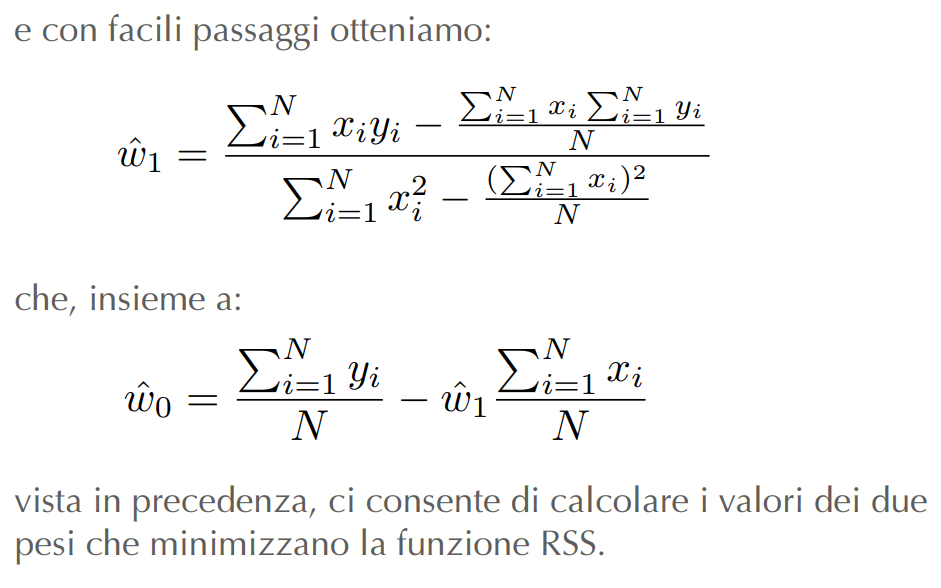
\includegraphics[width=\linewidth]{Screenshot 2024-12-11 165128.png} % Percorso dell'immagine
       % \caption{Arrivo in precedenza del processo più grande} % Didascalia per la seconda immagine
        \label{fig:destra} % Etichetta per riferimento
    \end{subfigure}
   % \caption{SJF/Shortest Job First} % Didascalia generale per la figura
    \label{fig:due_immagini} % Etichetta generale per riferimento
\end{figure}
\subsubsection{Gradient Descent}
Con questo approccio dobbiamo aggiornare i pesi in modo tale da spostarci nella direzione opposta al gradiente
\begin{figure}[H] % 'h' per indicare di posizionare la figura qui
    \centering % Centra l'intera figura
    % Immagine di sinistra
    \begin{subfigure}[t]{0.46\textwidth} % Sottotitolo di dimensione 45% della larghezza
        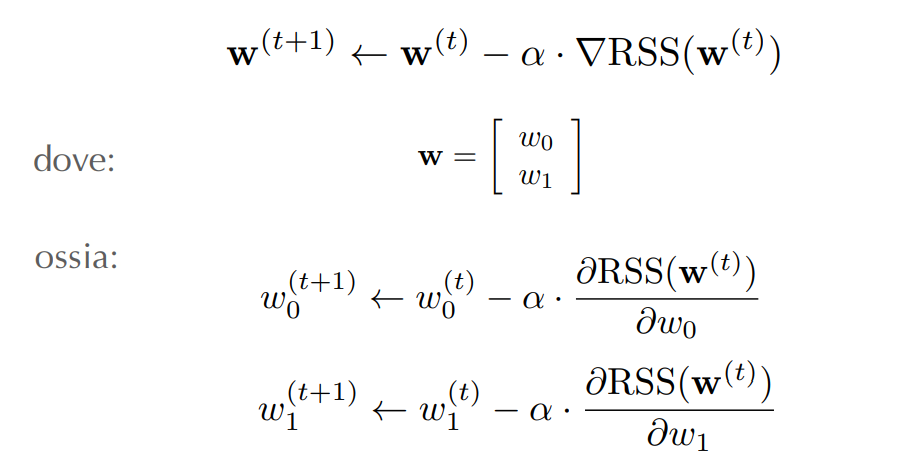
\includegraphics[width=\linewidth]{Screenshot 2024-12-11 165534.png} % Percorso dell'immagine
       % \caption{Arrivo in precedenza dei processi più piccoli} % Didascalia per la prima immagine
        \label{fig:sinistra} % Etichetta per riferimento
    \end{subfigure}
    \hspace{0.05\textwidth} % Spazio orizzontale tra le immagini
    % Immagine di destra
    \begin{subfigure}[t]{0.46\textwidth} % Sottotitolo di dimensione 45% della larghezza
        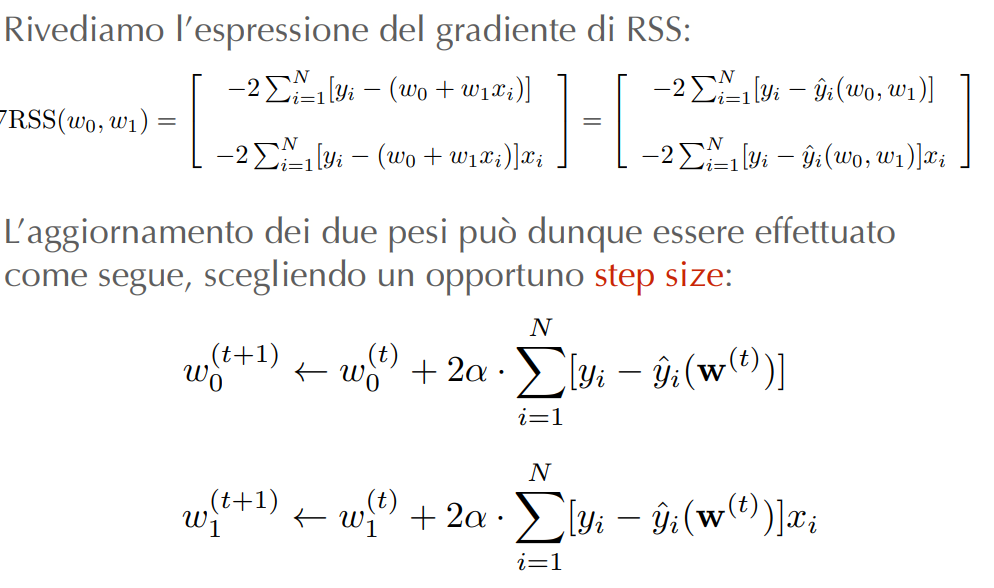
\includegraphics[width=\linewidth]{Screenshot 2024-12-11 165723.png} % Percorso dell'immagine
       % \caption{Arrivo in precedenza del processo più grande} % Didascalia per la seconda immagine
        \label{fig:destra} % Etichetta per riferimento
    \end{subfigure}
   % \caption{SJF/Shortest Job First} % Didascalia generale per la figura
    \label{fig:due_immagini} % Etichetta generale per riferimento
\end{figure}
\noindent
\vspace{150pt}
Dobbiamo infine scegliere un \textbf{criterio di convergenza}. Come già detto, per funzioni convesse si ha un minimo globale quando il gradiente è uguale a zero. In pratica possiamo fermarci quando:
\begin{figure}[H] % Usa 'H' per forzare la posizione qui
    \centering % Centra l'immagine
    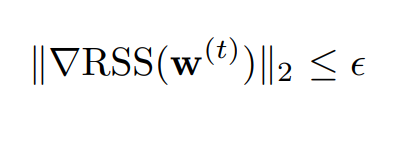
\includegraphics[width=5cm, height=2cm]{immagine_2024-12-11_170057411.png} % Percorso dell'immagine
    \caption{} % Didascalia per l'immagine
    \label{fig:immagine} % Etichetta per riferimento
\end{figure}
\noindent
\begin{figure}[H] % Usa 'H' per forzare la posizione qui
    \centering % Centra l'immagine
    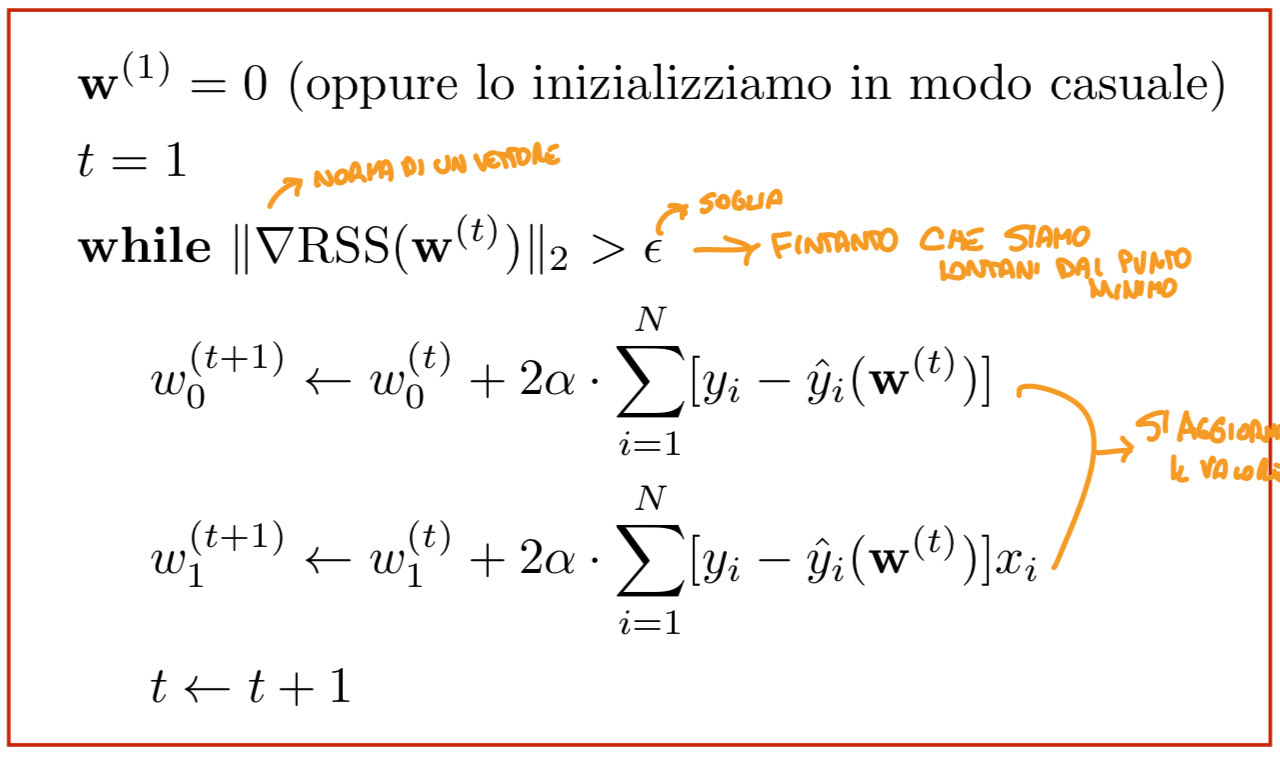
\includegraphics[width=10cm, height=6cm]{IMG_0839.jpeg} % Percorso dell'immagine
    \caption{} % Didascalia per l'immagine
    \label{fig:immagine} % Etichetta per riferimento
\end{figure}
\subsection{Multiple Regression (Linear Regression con Multiple Features)}
Fino ad ora abbiamo ipotizzato, per la funzione f(x), un andamento lineare per il nostro caso di studio relativo ai prezzi degli appartamenti. Tuttavia l'esperienza comune ci induce a pensare che la relazione tra le due variabili (area e prezzo di un appartamento) non sia proprio lineare. In genere, all'aumentare della metratura il prezzo aumenta ma non in modo esattamente proporzionale. Potremmo ipotizzare ad esempio una funzione quadratica o addirittura polinomiale di grado p
\begin{figure}[H] % Usa 'H' per forzare la posizione qui
    \centering % Centra l'immagine
    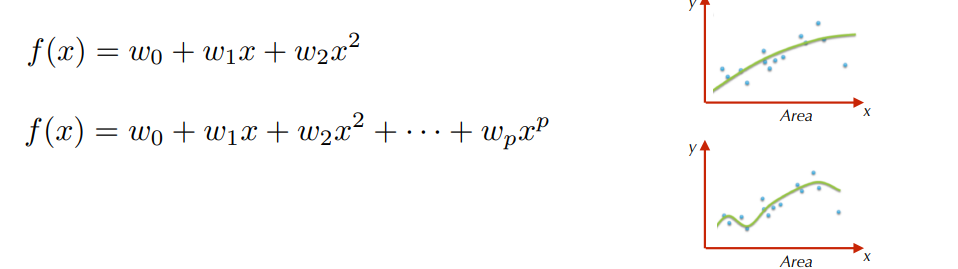
\includegraphics[width=12cm, height=4cm]{immagine_2024-12-11_173214015.png} % Percorso dell'immagine
    \caption{} % Didascalia per l'immagine
    \label{fig:immagine} % Etichetta per riferimento
\end{figure}
\noindent
In quest'ultimo caso avremmo una \textbf{Polinomial Regression} il cui modello è il seguente:
\begin{figure}[H] % 'h' per indicare di posizionare la figura qui
    \centering % Centra l'intera figura
    % Immagine di sinistra
    \begin{subfigure}[t]{0.46\textwidth} % Sottotitolo di dimensione 45% della larghezza
        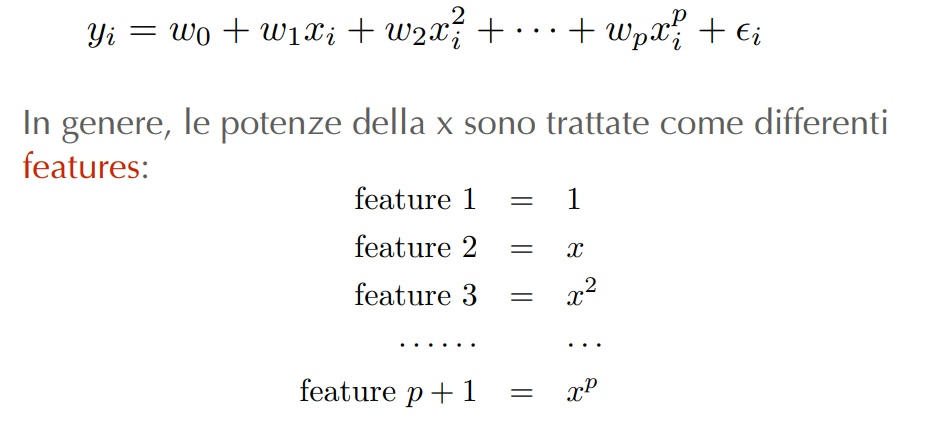
\includegraphics[width=\linewidth]{Screenshot 2024-12-11 173531.png} % Percorso dell'immagine
       % \caption{Arrivo in precedenza dei processi più piccoli} % Didascalia per la prima immagine
        \label{fig:sinistra} % Etichetta per riferimento
    \end{subfigure}
    \hspace{0.05\textwidth} % Spazio orizzontale tra le immagini
    % Immagine di destra
    \begin{subfigure}[t]{0.46\textwidth} % Sottotitolo di dimensione 45% della larghezza
        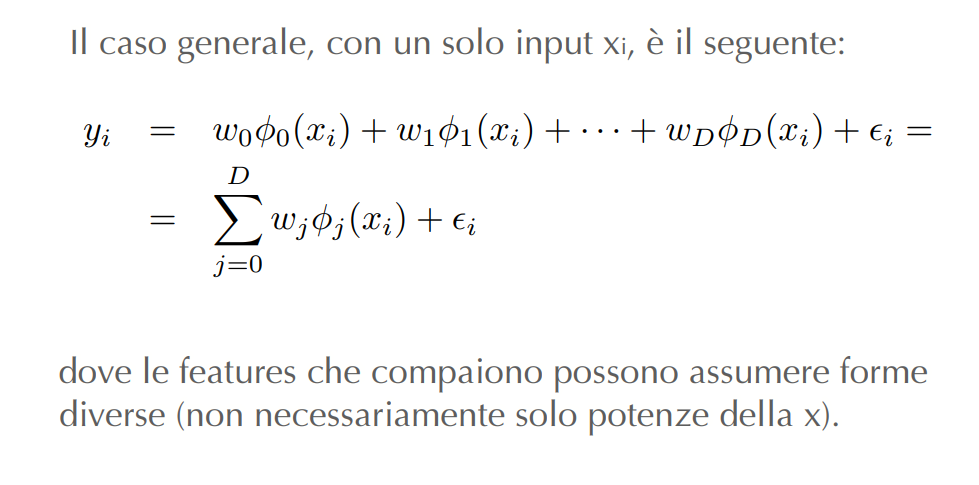
\includegraphics[width=\linewidth]{Screenshot 2024-12-11 173542.png} % Percorso dell'immagine
       % \caption{Arrivo in precedenza del processo più grande} % Didascalia per la seconda immagine
        \label{fig:destra} % Etichetta per riferimento
    \end{subfigure}
   % \caption{SJF/Shortest Job First} % Didascalia generale per la figura
    \label{fig:due_immagini} % Etichetta generale per riferimento
\end{figure}
\noindent
Se volessimo considerare anche altre caratteristiche in input avremmo un vettore $x_i$ per ogni esempio noto, le cui componenti sono appunto l'area, i bagni ecc...\\
Anche in questo caso possiamo utilizzare, come funzione di costo da minimizzare, la \textbf{RSS} definita come segue, a partire da N osservazioni disponibili:
\begin{figure}[H] % Usa 'H' per forzare la posizione qui
    \centering % Centra l'immagine
    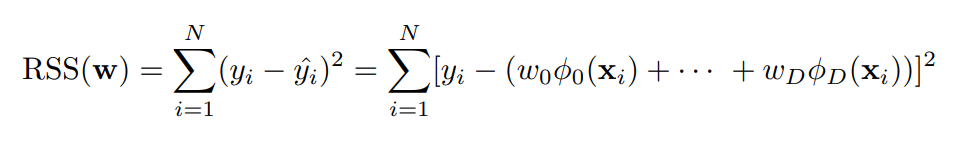
\includegraphics[width=14cm, height=2cm]{Screenshot 2024-12-11 174136.png} % Percorso dell'immagine
    \caption{} % Didascalia per l'immagine
    \label{fig:immagine} % Etichetta per riferimento
\end{figure}
\noindent
Il problema di addestrare il nostro modello è dunque quello di trovare i valori dei pesi \( \hat{w_0} \), \( \hat{w_1} \), ..., \( \hat{w_D} \) che minimizzano la funzione RSS (convessa anche in questo caso)
\subsubsection{Il processo di Training}
\begin{figure}[H] % Usa 'H' per forzare la posizione qui
    \centering % Centra l'immagine
    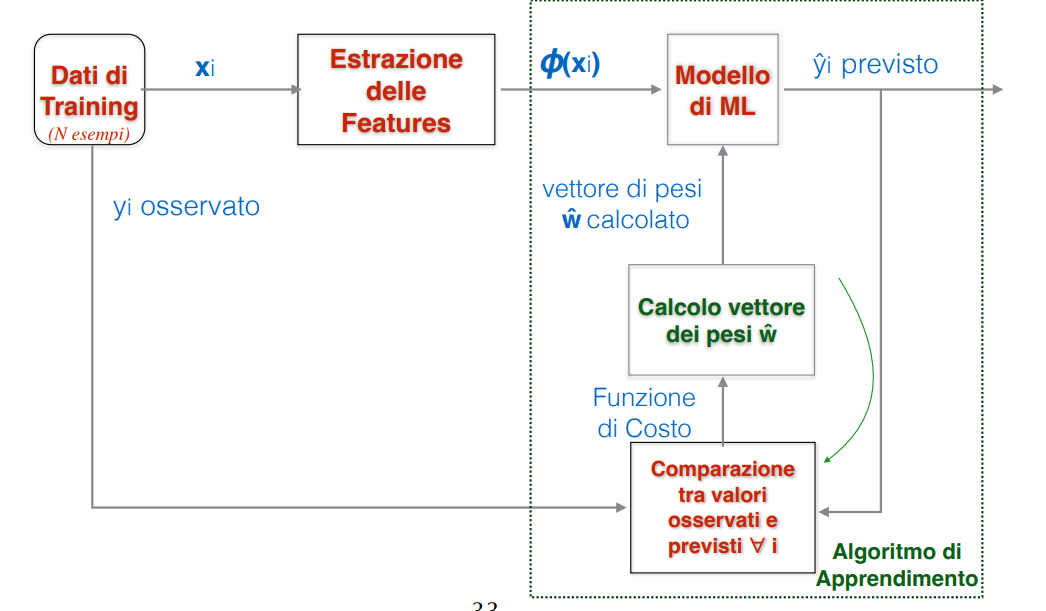
\includegraphics[width=11cm, height=7cm]{Screenshot 2024-12-11 174725.png} % Percorso dell'immagine
    \caption{} % Didascalia per l'immagine
    \label{fig:immagine} % Etichetta per riferimento
\end{figure}
\vspace{150pt}
\subsection{Regression Model in notazione Matriciale}
In molti casi può essere conveniente usare una notazione matriciale. L'espressione:
\begin{figure}[H] % Usa 'H' per forzare la posizione qui
    \centering % Centra l'immagine
    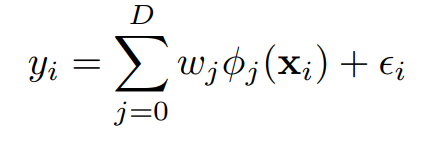
\includegraphics[width=8cm, height=2cm]{Screenshot 2024-12-11 174950.png} % Percorso dell'immagine
    \caption{} % Didascalia per l'immagine
    \label{fig:immagine} % Etichetta per riferimento
\end{figure}
Può essere riscritta:
\begin{figure}[H] % 'h' per indicare di posizionare la figura qui
    \centering % Centra l'intera figura
    % Immagine di sinistra
    \begin{subfigure}[t]{0.46\textwidth} % Sottotitolo di dimensione 45% della larghezza
        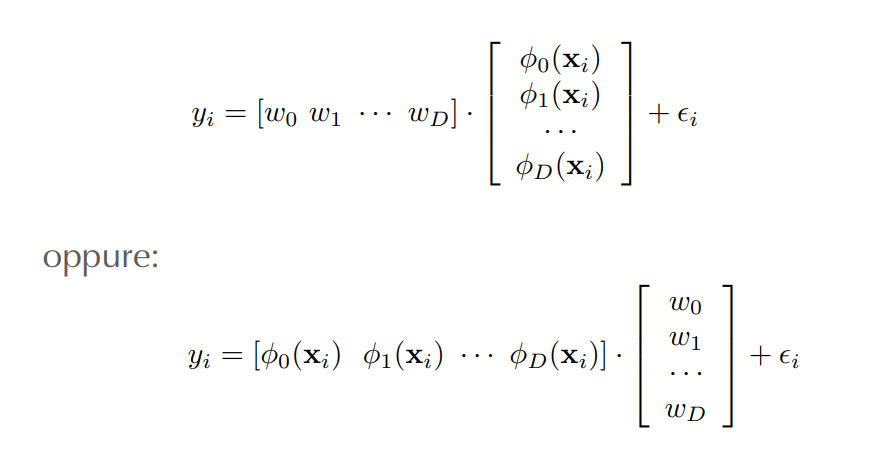
\includegraphics[width=\linewidth]{Screenshot 2024-12-11 175126.png} % Percorso dell'immagine
       % \caption{Arrivo in precedenza dei processi più piccoli} % Didascalia per la prima immagine
        \label{fig:sinistra} % Etichetta per riferimento
    \end{subfigure}
    \hspace{0.05\textwidth} % Spazio orizzontale tra le immagini
    % Immagine di destra
    \begin{subfigure}[t]{0.46\textwidth} % Sottotitolo di dimensione 45% della larghezza
        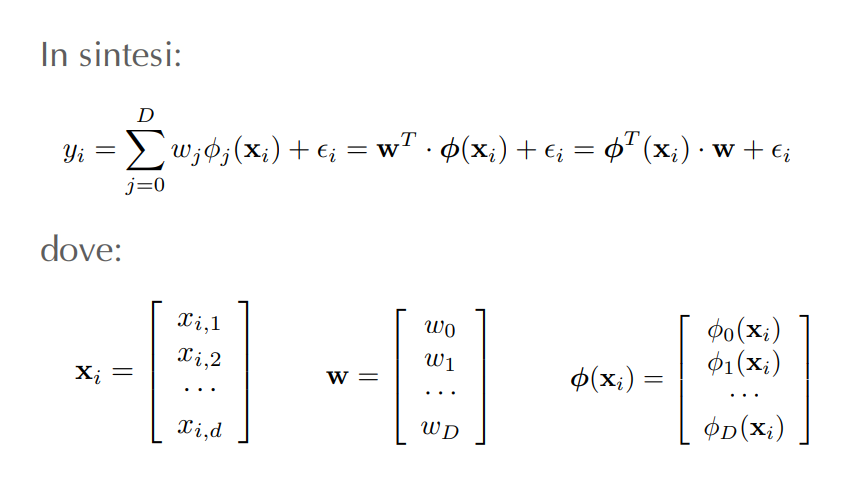
\includegraphics[width=\linewidth]{Screenshot 2024-12-11 175135.png} % Percorso dell'immagine
       % \caption{Arrivo in precedenza del processo più grande} % Didascalia per la seconda immagine
        \label{fig:destra} % Etichetta per riferimento
    \end{subfigure}
   % \caption{SJF/Shortest Job First} % Didascalia generale per la figura
    \label{fig:due_immagini} % Etichetta generale per riferimento
\end{figure}
\begin{figure}[H] % 'h' per indicare di posizionare la figura qui
    \centering % Centra l'intera figura
    % Immagine di sinistra
    \begin{subfigure}[t]{0.46\textwidth} % Sottotitolo di dimensione 45% della larghezza
        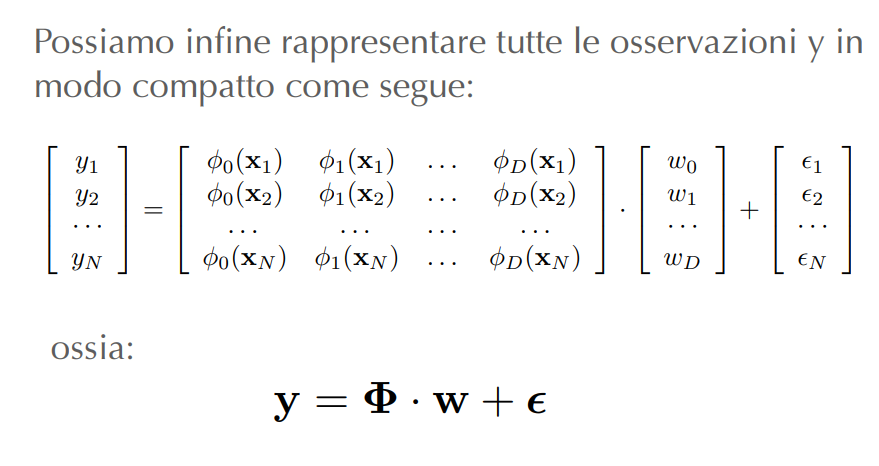
\includegraphics[width=\linewidth]{Screenshot 2024-12-11 175146.png} % Percorso dell'immagine
       % \caption{Arrivo in precedenza dei processi più piccoli} % Didascalia per la prima immagine
        \label{fig:sinistra} % Etichetta per riferimento
    \end{subfigure}
    \hspace{0.05\textwidth} % Spazio orizzontale tra le immagini
    % Immagine di destra
    \begin{subfigure}[t]{0.46\textwidth} % Sottotitolo di dimensione 45% della larghezza
        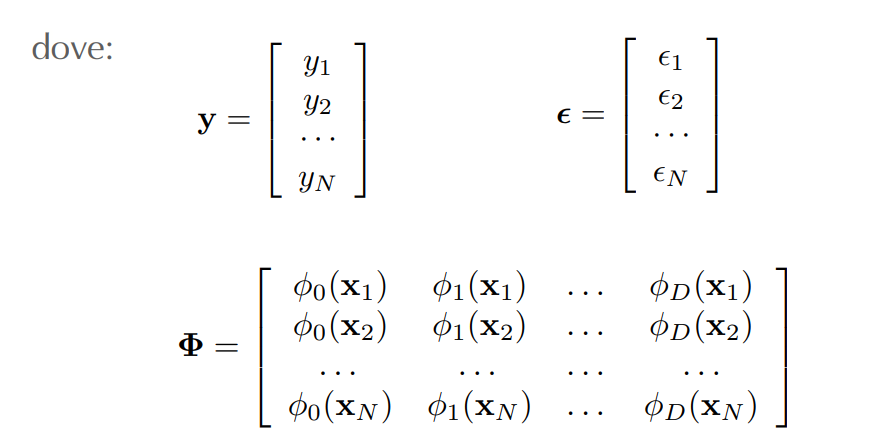
\includegraphics[width=\linewidth]{Screenshot 2024-12-11 175200.png} % Percorso dell'immagine
       % \caption{Arrivo in precedenza del processo più grande} % Didascalia per la seconda immagine
        \label{fig:destra} % Etichetta per riferimento
    \end{subfigure}
   % \caption{SJF/Shortest Job First} % Didascalia generale per la figura
    \label{fig:due_immagini} % Etichetta generale per riferimento
\end{figure}
\begin{figure}[H] % 'h' per indicare di posizionare la figura qui
    \centering % Centra l'intera figura
    % Immagine di sinistra
    \begin{subfigure}[t]{0.60\textwidth} % Sottotitolo di dimensione 45% della larghezza
        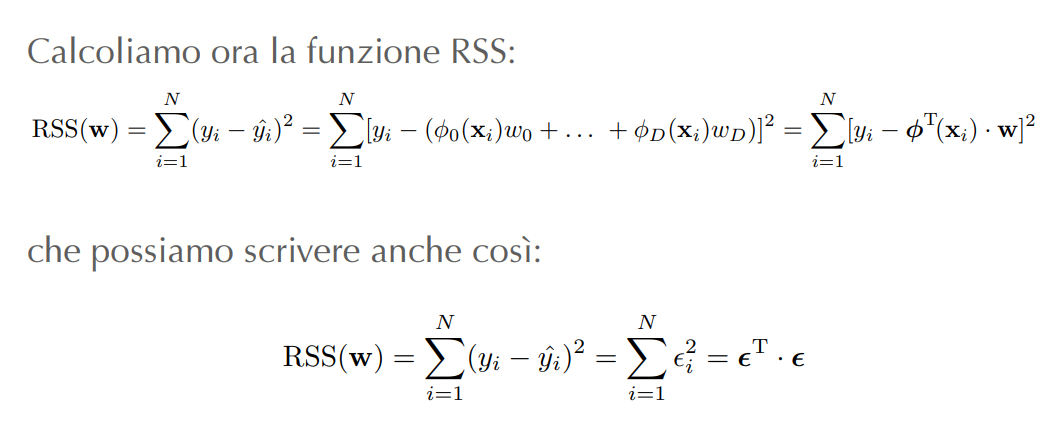
\includegraphics[width=\linewidth]{Screenshot 2024-12-11 175221.png} % Percorso dell'immagine
       % \caption{Arrivo in precedenza dei processi più piccoli} % Didascalia per la prima immagine
        \label{fig:sinistra} % Etichetta per riferimento
    \end{subfigure}
    \hspace{0.05\textwidth} % Spazio orizzontale tra le immagini
    % Immagine di destra
    \begin{subfigure}[t]{0.60\textwidth} % Sottotitolo di dimensione 45% della larghezza
        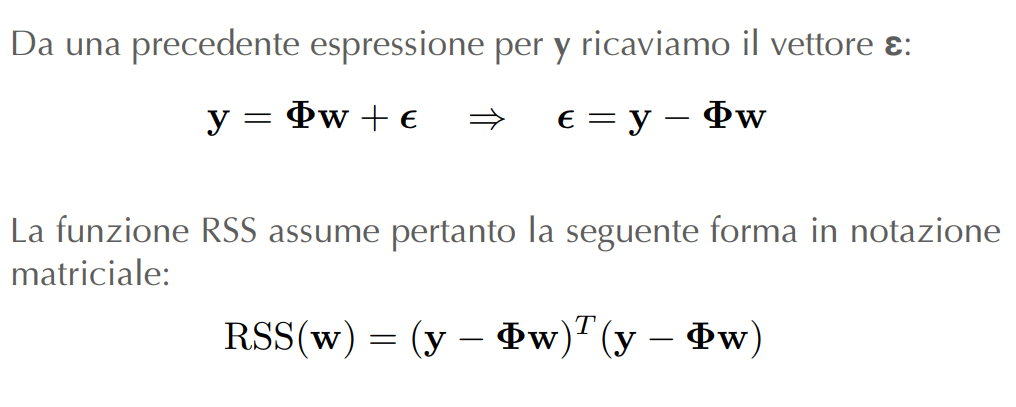
\includegraphics[width=\linewidth]{Screenshot 2024-12-11 175238.png} % Percorso dell'immagine
       % \caption{Arrivo in precedenza del processo più grande} % Didascalia per la seconda immagine
        \label{fig:destra} % Etichetta per riferimento
    \end{subfigure}
   % \caption{SJF/Shortest Job First} % Didascalia generale per la figura
    \label{fig:due_immagini} % Etichetta generale per riferimento
\end{figure}
\noindent
\subsubsection{Gradiente della funzione RSS}
Calcoliamo ora il gradiente della funzione RSS, partendo dalla precedente espressione matriciale.
\begin{figure}[H] % Usa 'H' per forzare la posizione qui
    \centering % Centra l'immagine
    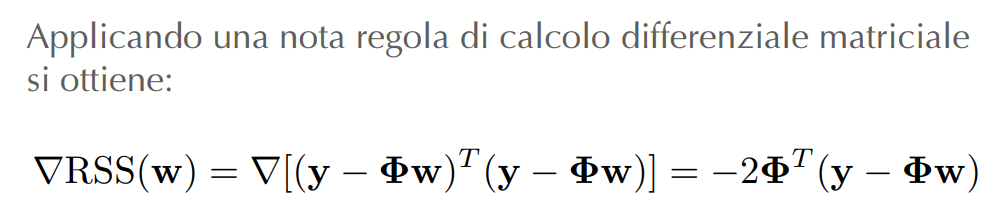
\includegraphics[width=13cm, height=3cm]{Screenshot 2024-12-11 175936.png} % Percorso dell'immagine
    \caption{} % Didascalia per l'immagine
    \label{fig:immagine} % Etichetta per riferimento
\end{figure}
\vspace{200pt}
\subsubsection{Forma Chiusa}
\begin{figure}[H] % Usa 'H' per forzare la posizione qui
    \centering % Centra l'immagine
    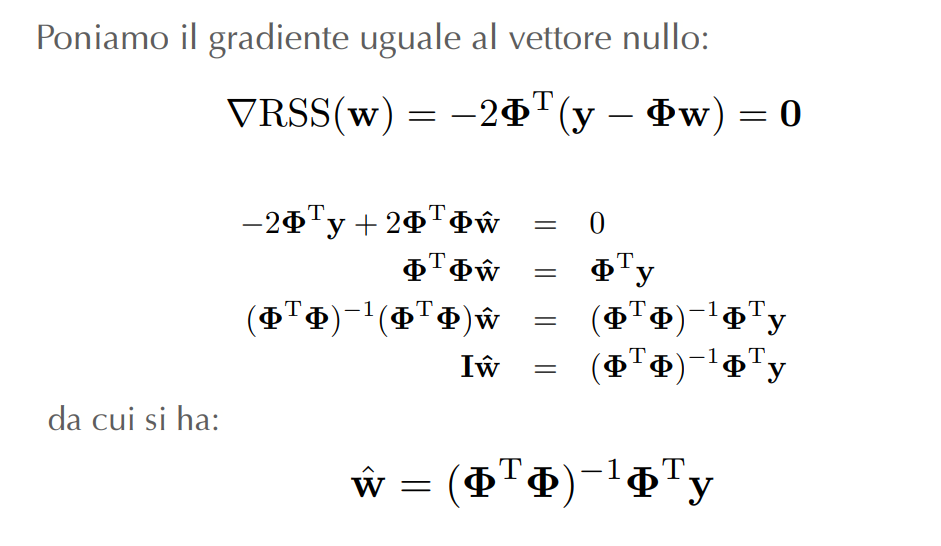
\includegraphics[width=13cm, height=6cm]{Screenshot 2024-12-11 180347.png} % Percorso dell'immagine
    \caption{} % Didascalia per l'immagine
    \label{fig:immagine} % Etichetta per riferimento
\end{figure}
\subsubsection{Gradient Descent}
\begin{figure}[H] % 'h' per indicare di posizionare la figura qui
    \centering % Centra l'intera figura
    % Immagine di sinistra
    \begin{subfigure}[t]{0.60\textwidth} % Sottotitolo di dimensione 45% della larghezza
        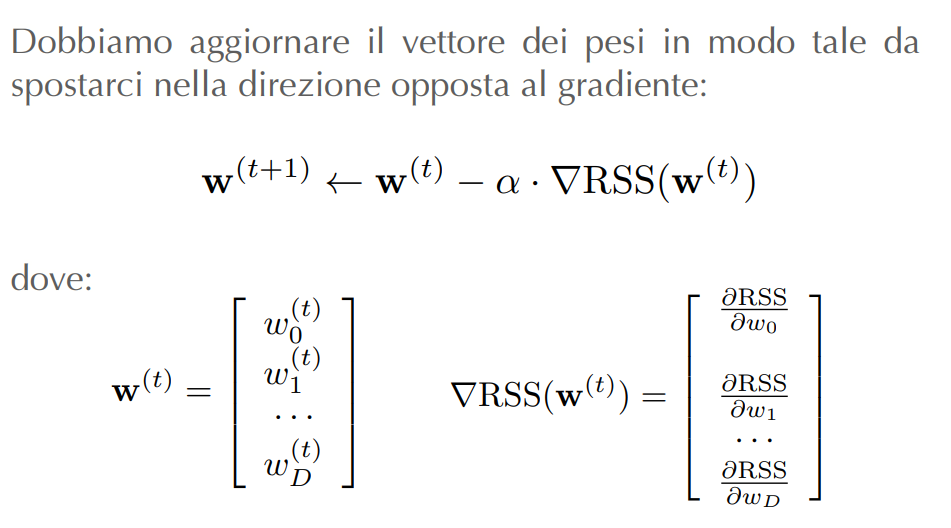
\includegraphics[width=\linewidth]{Screenshot 2024-12-11 180816.png} % Percorso dell'immagine
       % \caption{Arrivo in precedenza dei processi più piccoli} % Didascalia per la prima immagine
        \label{fig:sinistra} % Etichetta per riferimento
    \end{subfigure}
    \hspace{0.05\textwidth} % Spazio orizzontale tra le immagini
    % Immagine di destra
    \begin{subfigure}[t]{0.60\textwidth} % Sottotitolo di dimensione 45% della larghezza
        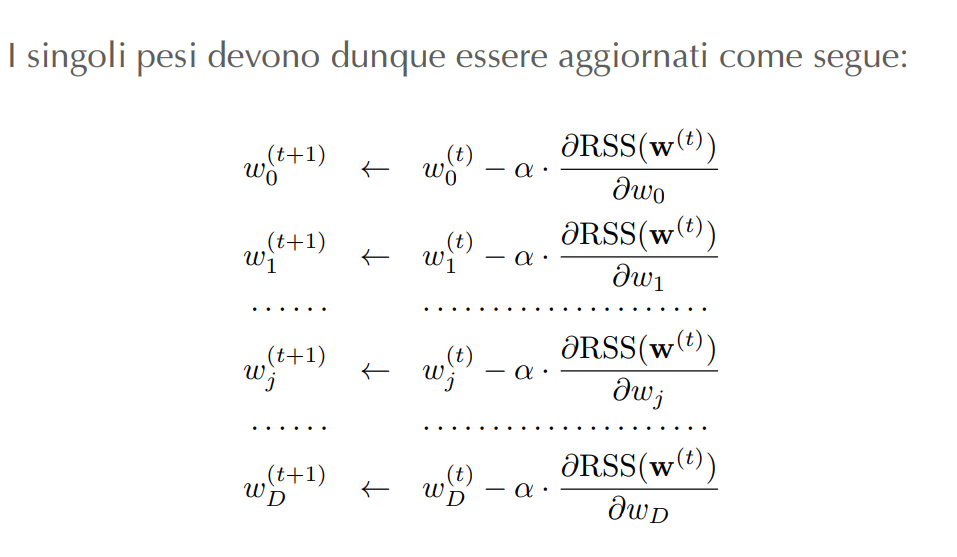
\includegraphics[width=\linewidth]{Screenshot 2024-12-11 180824.png} % Percorso dell'immagine
       % \caption{Arrivo in precedenza del processo più grande} % Didascalia per la seconda immagine
        \label{fig:destra} % Etichetta per riferimento
    \end{subfigure}
   % \caption{SJF/Shortest Job First} % Didascalia generale per la figura
    \label{fig:due_immagini} % Etichetta generale per riferimento
\end{figure}
\noindent
\begin{figure}[H] % Usa 'H' per forzare la posizione qui
    \centering % Centra l'immagine
    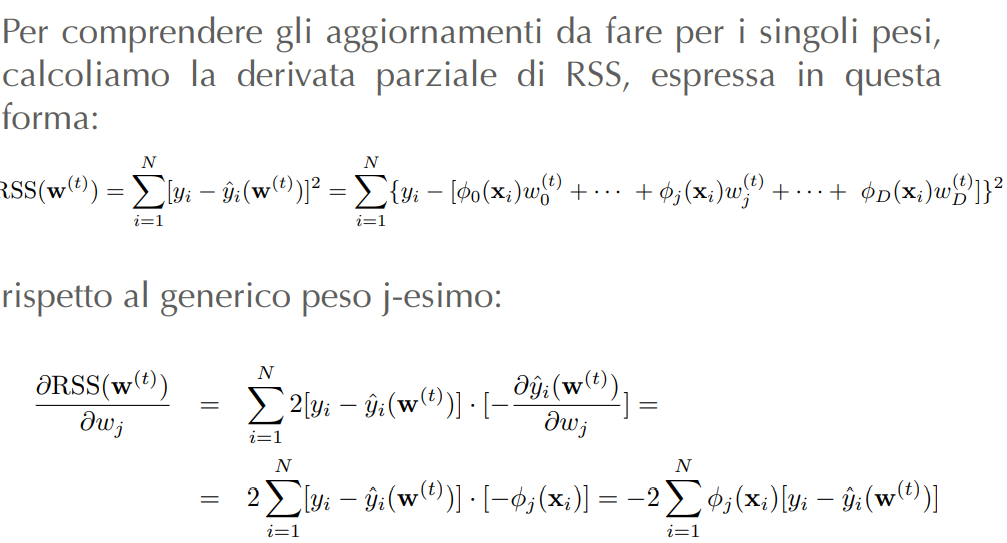
\includegraphics[width=11cm, height=7cm]{Screenshot 2024-12-11 180834.png} % Percorso dell'immagine
    \caption{} % Didascalia per l'immagine
    \label{fig:immagine} % Etichetta per riferimento
\end{figure}
\noindent
Anche in questo caso dobbiamo scegliere un criterio di convergenza, quello scelto per il caso singolo va bene.
\begin{figure}[H] % Usa 'H' per forzare la posizione qui
    \centering % Centra l'immagine
    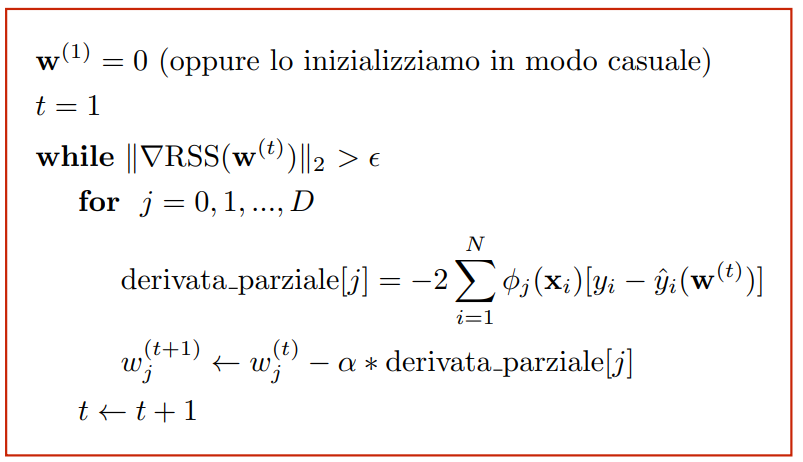
\includegraphics[width=12cm, height=7cm]{Screenshot 2024-12-11 193835.png} % Percorso dell'immagine
    \caption{} % Didascalia per l'immagine
    \label{fig:immagine} % Etichetta per riferimento
\end{figure}
\subsection{Workflow per Regression}
I due task importanti che dobbiamo attuare nella regression sono: scelta del modello di regressione (\textbf{model selection}), valutazione del modello (\textbf{model assessment}).\\
Nel \textbf{Model selection} scegliamo dei parametri di tuning $\lambda$ che controllano la complessità del modello (es. grado del polinomio). Nel \textbf{Model assessment} effettuiamo la valutazione del Generalization Error (o True Error)\\
Ovviamente è importante evitare il peaking, ovvero non bisogna selezionare le ipotesi in base alle sue prestazioni sull'insieme di test e l'overfitting, ovvero strutturare tutto sulla base dei dati in possesso. 
\begin{figure}[H] % Usa 'H' per forzare la posizione qui
    \centering % Centra l'immagine
    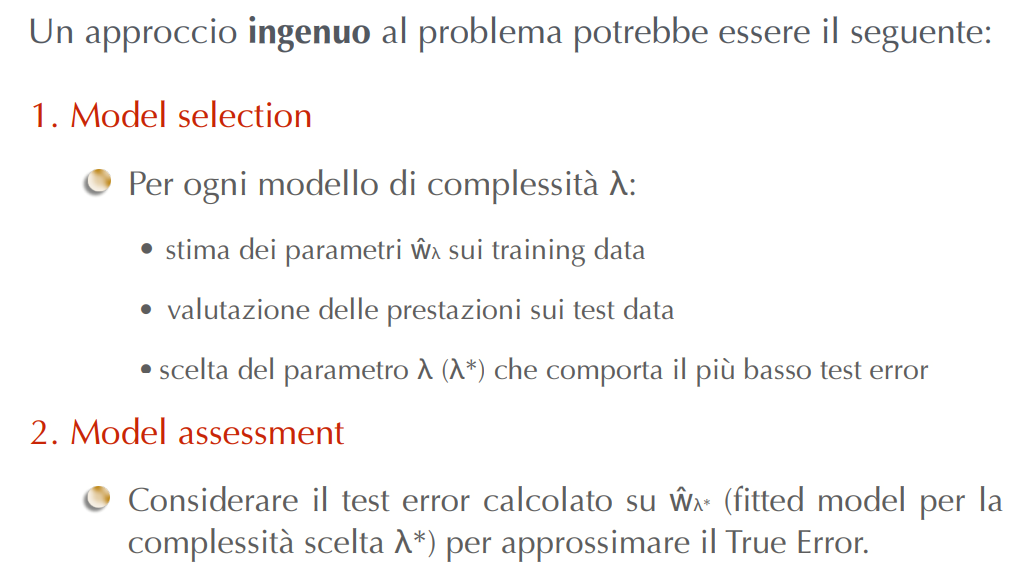
\includegraphics[width=12cm, height=7cm]{Screenshot 2024-12-11 194754.png} % Percorso dell'immagine
    \caption{} % Didascalia per l'immagine
    \label{fig:immagine} % Etichetta per riferimento
\end{figure}
\begin{figure}[H] % Usa 'H' per forzare la posizione qui
    \centering % Centra l'immagine
    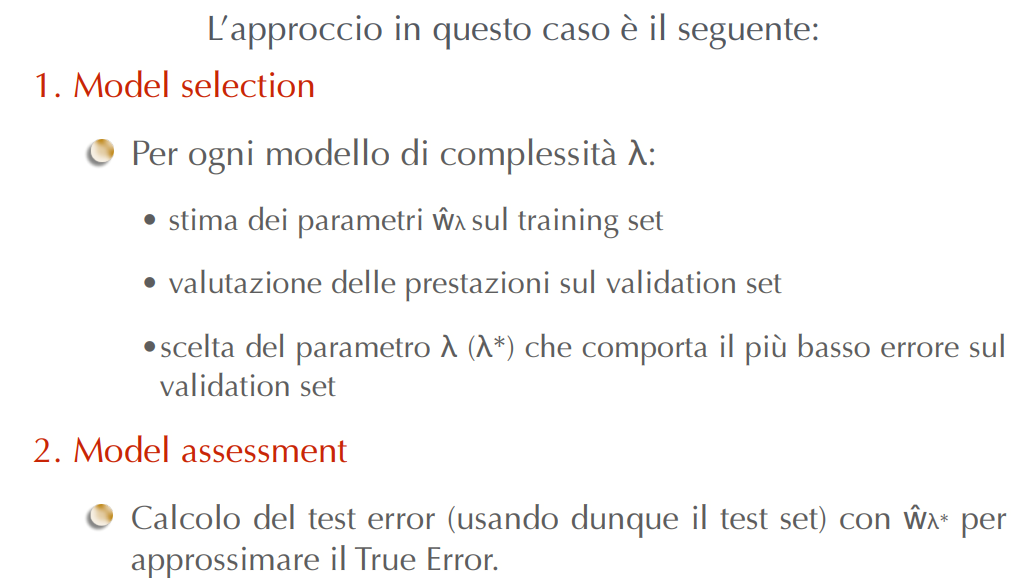
\includegraphics[width=12cm, height=7cm]{Screenshot 2024-12-11 194805.png} % Percorso dell'immagine
    \caption{} % Didascalia per l'immagine
    \label{fig:immagine} % Etichetta per riferimento
\end{figure}
\begin{figure}[H] % Usa 'H' per forzare la posizione qui
    \centering % Centra l'immagine
    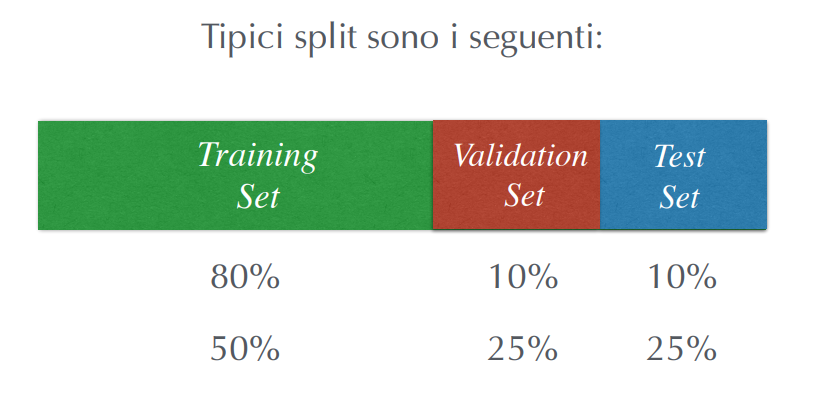
\includegraphics[width=12cm, height=4cm]{Screenshot 2024-12-11 195230.png} % Percorso dell'immagine
    \caption{} % Didascalia per l'immagine
    \label{fig:immagine} % Etichetta per riferimento
\end{figure}
\section{Regressione Errori}
\subsection{Valutazione delle Prestazioni}
La valutazione degli errori delle prestazioni è di importanza cruciale per poter apprezzare il metodo che stiamo utilizzando per le nostre previsioni. Essa ci aiuta nella scelta tra modelli di diversa complessità a nostra disposizione. A tal fine occorre definire una metrica che ci consenta di valutare quanto perdiamo (loss) quando facciamo una certa previsione.
\subsection{Loss Function}
Possiamo indicare una funzione di Loss come segue:
\begin{figure}[H] % Usa 'H' per forzare la posizione qui
    \centering % Centra l'immagine
    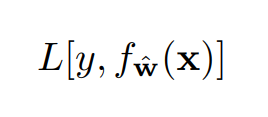
\includegraphics[width=4cm, height=2cm]{Screenshot 2024-12-12 130339.png} % Percorso dell'immagine
    \caption{} % Didascalia per l'immagine
    \label{fig:immagine} % Etichetta per riferimento
\end{figure}
\noindent
Dove y è l'actual value, mentre la funzione f ci fornisce il valore previsto \textbf{\( \hat{y} \)}. Tale funzione L rappresenta il costo che abbiamo se usiamo la f con il vettore dei pesi \( \hat{w} \) a fronte dell'input x. In pratica la Loss Function quantifica quanto è lontana la previsione del modello dai valori reali. La Loss Function viene utilizzata durante il training per aggiornare i pesi \( \hat{w} \) della funzione f. Lo scopo è minimizzare la funzione di perdita, così il modello fornirà previsioni migliori.
\subsubsection{Esempi di Loss Function}
\begin{figure}[H] % Usa 'H' per forzare la posizione qui
    \centering % Centra l'immagine
    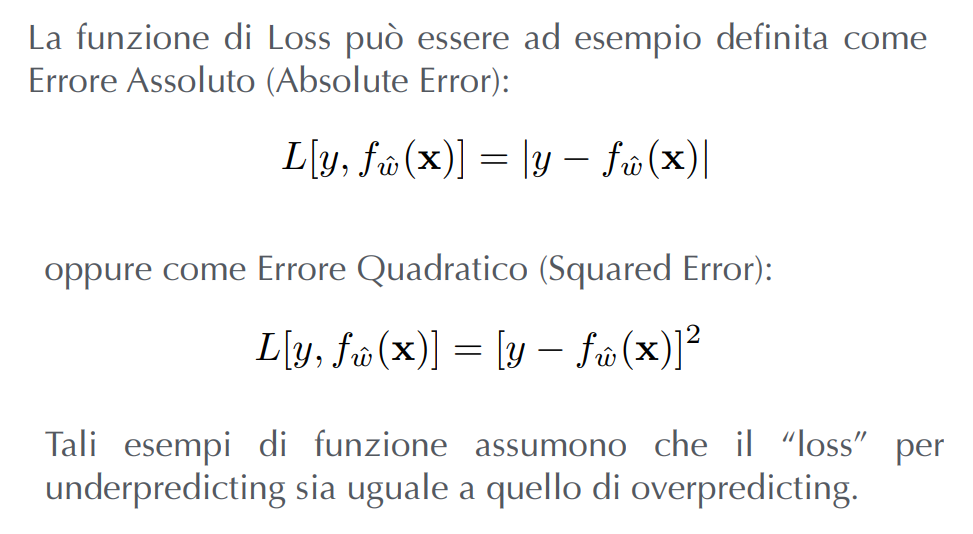
\includegraphics[width=10cm, height=5cm]{Screenshot 2024-12-12 131423.png} % Percorso dell'immagine
    \caption{} % Didascalia per l'immagine
    \label{fig:immagine} % Etichetta per riferimento
\end{figure}
\vspace{300pt}
\subsection{Le tre misure di Loss}
\subsubsection{Training Error}
Il \textbf{training error} è la media degli errori calcolati con la funzione di perdita (L) sui dati del training set.
Consideriamo ancora l'esempio relativo ai prezzi degli appartamenti. Supponiamo di avere a disposizione le osservazioni come rappresentate in figura (puntini blu). Dobbiamo decidere un modello da utilizzare e scegliere un sotto insieme delle osservazioni per effettuare la fase di training del modello. Possiamo ad esempio scegliere un modello quadratico e calcolare i pesi w tali da minimizzare la funzione RSS
\begin{figure}[H] % Usa 'H' per forzare la posizione qui
    \centering % Centra l'immagine
    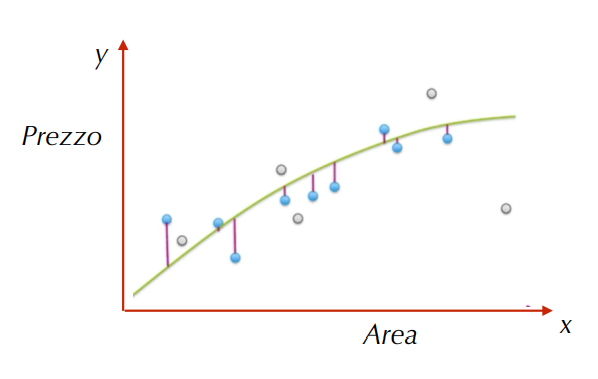
\includegraphics[width=10cm, height=5cm]{Screenshot 2024-12-12 131848.png} % Percorso dell'immagine
    \caption{} % Didascalia per l'immagine
    \label{fig:immagine} % Etichetta per riferimento
\end{figure}
\noindent
Una volta stimmati i parametri del modello, possiamo valutare il training error di tale modello stimato come segue: Definizione di una Loss Function e Calcolo del Training Error come "Average Loss", definito sugli N punti di training:
\begin{figure}[H] % Usa 'H' per forzare la posizione qui
    \centering % Centra l'immagine
    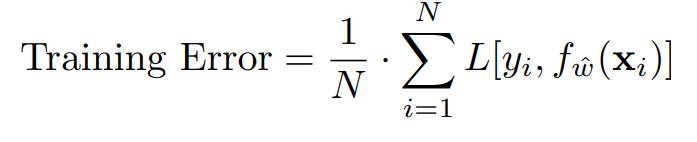
\includegraphics[width=10cm, height=2cm]{immagine_2024-12-12_132135090.png} % Percorso dell'immagine
    \caption{} % Didascalia per l'immagine
    \label{fig:immagine} % Etichetta per riferimento
\end{figure}
\noindent
Più è complesso il modello e minore sarà l'errore. Il Training Error in generale non è una buona misura dato che è eccessivamente ottimistico, proprio perchè il vettore \( \hat{w} \) è calcolato affinchè il modello si adatti ai dati di training. 
\begin{figure}[H] % Usa 'H' per forzare la posizione qui
    \centering % Centra l'immagine
    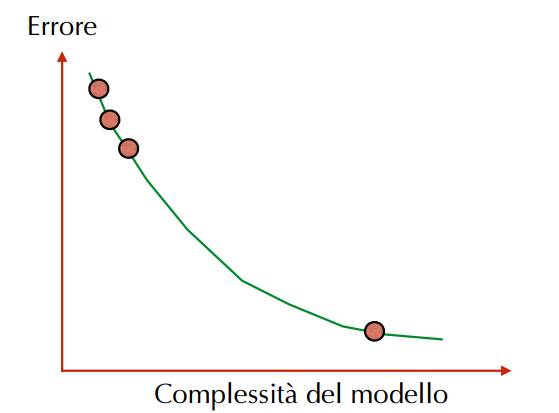
\includegraphics[width=10cm, height=5cm]{Screenshot 2024-12-12 132622.png} % Percorso dell'immagine
    \caption{} % Didascalia per l'immagine
    \label{fig:immagine} % Etichetta per riferimento
\end{figure}
\subsubsection{Generalization Error}
Il generalization error (o errore di generalizzazione) misura quanto bene un modello addestrato riesce a fare previsioni accurate su dati nuovi e mai visti prima, cioè al di fuori del training set. Sarebbe interessante conoscere il "loss" prendendo in considerazione tutte le possibili coppie (x, y) ossia, per il nostro esempio degli appartamenti, tutte le possibili case della zona presa in considerazione, calcolando la media della funzione loss su tali appartamenti. In genere però nel nostro data set abbiamo soltato un numero limitato di osservazioni (x,y). Per effettuare una stima di tale costo dovremmo cercare di pesare le varie coppie (x, y) in base alla probabilità che hanno di essere presenti nella zona d'interesse. Dunque è utile prendere in considerazione la distribuzione degli appartamenti in base al valore della loro area. Potremmo inoltre considerare la distribuzione delle case in base al loro prezzo, a parità di area.
\begin{figure}[H] % 'h' per indicare di posizionare la figura qui
    \centering % Centra l'intera figura
    % Immagine di sinistra
    \begin{subfigure}[t]{0.46\textwidth} % Sottotitolo di dimensione 45% della larghezza
        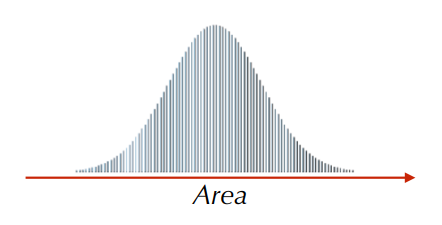
\includegraphics[width=\linewidth]{Screenshot 2024-12-12 140221.png} % Percorso dell'immagine
       % \caption{Arrivo in precedenza dei processi più piccoli} % Didascalia per la prima immagine
        \label{fig:sinistra} % Etichetta per riferimento
    \end{subfigure}
    \hspace{0.05\textwidth} % Spazio orizzontale tra le immagini
    % Immagine di destra
    \begin{subfigure}[t]{0.46\textwidth} % Sottotitolo di dimensione 45% della larghezza
        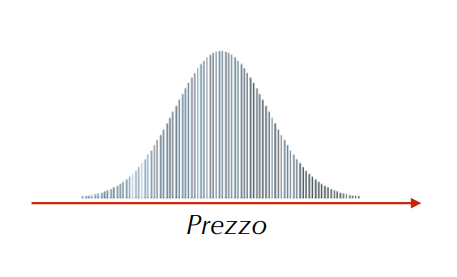
\includegraphics[width=\linewidth]{Screenshot 2024-12-12 140228.png} % Percorso dell'immagine
       % \caption{Arrivo in precedenza del processo più grande} % Didascalia per la seconda immagine
        \label{fig:destra} % Etichetta per riferimento
    \end{subfigure}
   % \caption{SJF/Shortest Job First} % Didascalia generale per la figura
    \label{fig:due_immagini} % Etichetta generale per riferimento
\end{figure}
\noindent
\begin{figure}[H] % Usa 'H' per forzare la posizione qui
    \centering % Centra l'immagine
    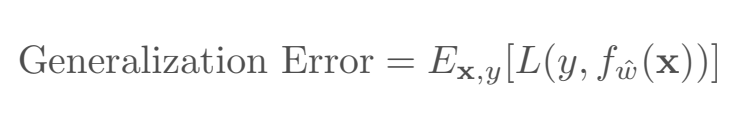
\includegraphics[width=10cm, height=2cm]{immagine_2024-12-12_140401158.png} % Percorso dell'immagine
    \caption{} % Didascalia per l'immagine
    \label{fig:immagine} % Etichetta per riferimento
\end{figure}
\noindent
Lo definiamo come l'average value della funzione Loss, calcolato su tutte le possibili coppie (x,y) pesate in base alla loro probabilità di comparire nella zona.
\begin{figure}[H] % Usa 'H' per forzare la posizione qui
    \centering % Centra l'immagine
    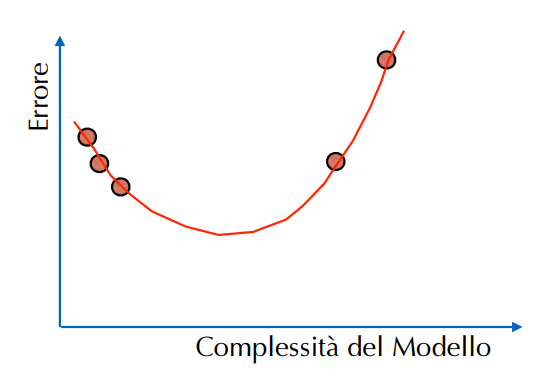
\includegraphics[width=6cm, height=4cm]{immagine_2024-12-12_140937502.png} % Percorso dell'immagine
    \caption{} % Didascalia per l'immagine
    \label{fig:immagine} % Etichetta per riferimento
\end{figure}
\noindent
C'è da ricordare che il Generalization Error non è calcolabile, per calcolarlo dovremmo conoscere la "true distribution" delle probabilità vista prima, cosa che non sappiamo fare.
\subsubsection{Test Error}
Il Test Error (o errore di test) è una misura dell'accuratezza di un modello su un test set, cioè un insieme di dati separato e mai usato durante l'addestramento o la validazione. È un'approssimazione empirica dell'errore di generalizzazione. Definito come average loss sui punti dell'insieme di test:
\begin{figure}[H] % Usa 'H' per forzare la posizione qui
    \centering % Centra l'immagine
    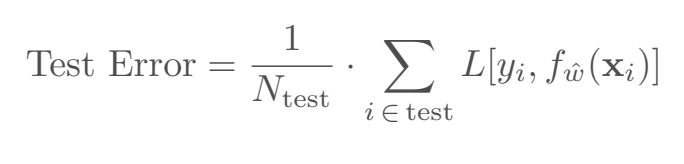
\includegraphics[width=8cm, height=2cm]{Screenshot 2024-12-12 141227.png} % Percorso dell'immagine
    \caption{} % Didascalia per l'immagine
    \label{fig:immagine} % Etichetta per riferimento
\end{figure}
\begin{figure}[H] % Usa 'H' per forzare la posizione qui
    \centering % Centra l'immagine
    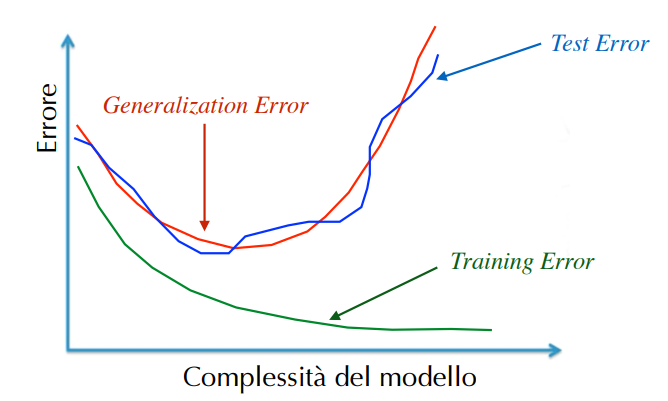
\includegraphics[width=7cm, height=5cm]{Screenshot 2024-12-12 141344.png} % Percorso dell'immagine
    \caption{} % Didascalia per l'immagine
    \label{fig:immagine} % Etichetta per riferimento
\end{figure}
\subsection{Overfitting}
Dato un modello con parametri \( \hat{w} \)\, si ha overfitting se esiste un modello con i parametri stimati w' tale che:
\begin{figure}[H] % Usa 'H' per forzare la posizione qui
    \centering % Centra l'immagine
    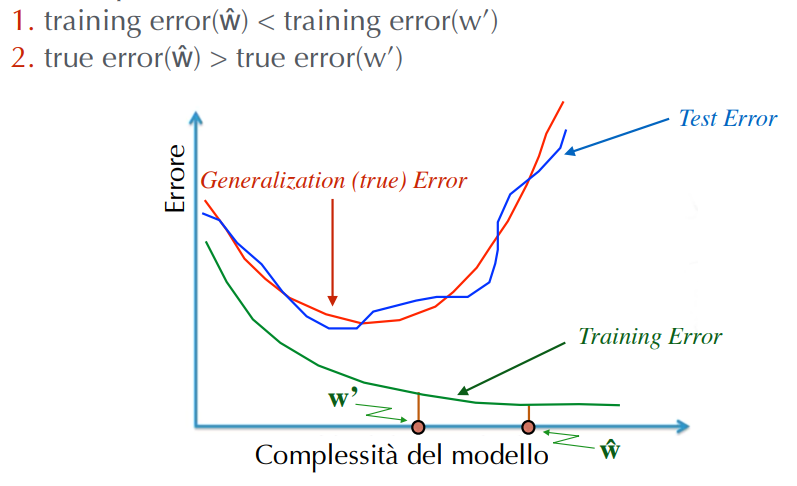
\includegraphics[width=9cm, height=7cm]{immagine_2024-12-12_141722009.png} % Percorso dell'immagine
    \caption{} % Didascalia per l'immagine
    \label{fig:immagine} % Etichetta per riferimento
\end{figure}
\section{\textcolor{red}{Classificatore di Bayes}}
\subsection{Introduzione}
Quando un agente conosce l'ambiente circostante, l'approccio logico gli consente di derivare piani efficaci. Ma gli agenti non hanno quasi mai accesso a tutta l'informazione necessaria: devono quindi agire in condizioni di \textbf{incertezza}. La \textbf{teoria della probabilità} è il modo migliore di ragionare in condizioni di incertezza.
\subsection{Approccio Bayesiano}
Il problema è posto in \textbf{termini probabilistici}. Se tutte le \textbf{distribuzioni in gioco sono note} l'\textbf{approccio Bayesiano} costituisce la migliore regola di classificazione possibile: \textbf{soluzione OTTIMA!}.\\\\
Sia \textbf{V} uno spazio di pattern \textbf{d}-dimensionali e $W = \{ w_1,w_2,...,w_s\}$ un insieme di \textbf{s} classi disgiunte costituite da elementi di \textbf{V}.\\
Per ogni \textbf{$x \in V$} e per ogni \textbf{$w_1 \in W$}, indichiamo con $p(x|w_i)$ la \textcolor{red}{\textbf{densità di probabilità condizionale}} di \textbf{x} data \textbf{$w_i$}, ovvero la densità di probabilità che il prossimo pattern sia \textbf{x} sotto l'ipotesi che la sua classe di appartenenza sia \textbf{$w_i$}. (Per un nuovo pattern x da classificare: si contano le occorrenze dei pattern del training set delle due classi in un intorno di \textbf{x} (vedi es maschi femmine) ($\frac{numPattAppartententiAllIntorno}{numPattAppartenentiAllaClasse}$))\\
Per ogni \textbf{$w_i \in W$}, indichiamo con \textbf{P($w_i$)} la \textcolor{red}{\textbf{probabilità a priori}} di $w_i$ ovvero la probabilità, indipendentemente dall'osservazione, che il prossimo pattern da classificare sia di classe \textbf{$w_i$}. (Si considera l'occorrenza dei pattern nel training set $\frac{numPattAppartententiAllaClasse}{numPattTotali}$)\\
Per ogni \textbf{$x \in V$} indichiamo con \textbf{p(x)} la \textbf{densità di probabilità assoluta} di \textbf{x}, ovvero la densità di probabilità che il prossimo pattern da classificare sia \textbf{x}
\begin{figure}[H] % Usa 'H' per forzare la posizione qui
    \centering % Centra l'immagine
    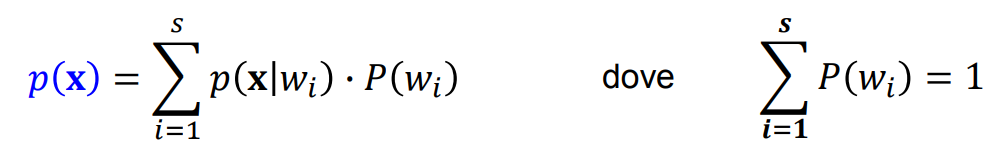
\includegraphics[width=11cm, height=2cm]{Screenshot 2024-12-12 151951.png} % Percorso dell'immagine
    \caption{} % Didascalia per l'immagine
    \label{fig:immagine} % Etichetta per riferimento
\end{figure}
\noindent
Per ogni \textbf{$w_i \in W$} e per ogni \textbf{$x \in V$} indichiamo con \textbf{$P(w_i|x)$} la \textcolor{red}{\textbf{probabilità a posteriori}} di \textbf{$w_i$} dato \textbf{x}, ovvero la probabilità che avendo osservato il pattern \textbf{x}, la classe di appartenenza sia \textbf{$w_i$}.
Per il \textcolor{red}{\textbf{teorema di Bayes}}:
$$\textcolor{red}{P(w_i|x)}=\frac{p(x|w_i)\cdot P(w_i)}{p(x)}$$
\subsection{Classificatore di Bayes}
Dato un pattern \textbf{x} da classificare in una delle \textbf{s} classi \textbf{$w_1,w_2,...,w_s$} di cui sono note: le \textbf{probabilità a priori} P($w_1$), ... e le \textbf{densità di probabilità condizionali} p($x|w_1$) ...\\
la \textcolor{red}{\textbf{regola di classificazione}} di Bayes assegna \textbf{x} alla classe \textbf{b} per cui è massima la probabilità a posteriori:
$$\textcolor{red}{b}=argmax_{i=1..s}\{ P(w_i|x)\}$$
\noindent
Massimizzare la probabilità a posteriori significa \textbf{massimizzare} la densità di probabilità condizionale tenendo comunque conto della probabilità a priori delle classi. (Per capire meglio guarda esempio maschi/femmine sulle slide)
\subsubsection{Esempio maschi femmine}
\begin{figure}[H] % Usa 'H' per forzare la posizione qui
    \centering % Centra l'immagine
    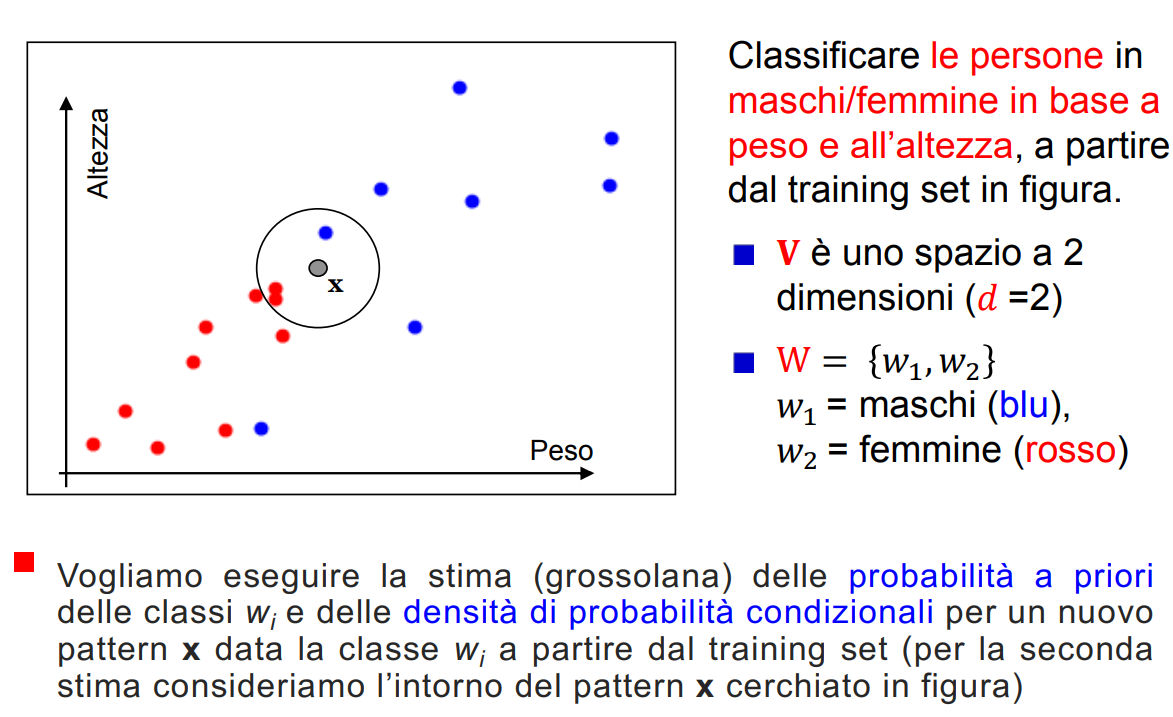
\includegraphics[width=10cm, height=6cm]{Screenshot 2024-12-12 155229.png} % Percorso dell'immagine
    \caption{} % Didascalia per l'immagine
    \label{fig:immagine} % Etichetta per riferimento
\end{figure}
\noindent
Una volta fatta la stima applichiamo il \textbf{teorema di Bayes} e facciammo la probabilità a posteriori. L'approccio Bayesiano assegnerà il pattern alla classe con probabilità a posteriori più alta (femmine).
\subsection{\textcolor{red}{Approcci parametrici e non}}
Mentre la stima delle probabilità a priori è abbastanza semplice \textbf{la conoscenza} delle densità condizionali è possibile "\textbf{solo in teoria}"; nella \textbf{pratica} due soluzioni:\\\\
\textcolor{red}{\textbf{Approccio parametrico}}: si fanno ipotesi sulla forma delle distribuzioni (es. \textbf{distribuzione multinormale}) e si apprendono i parametri fondamentali (\textbf{vettore medio, matrice di covarianza}) dal training set.\\
\textcolor{red}{\textbf{Approccio non parametrico}}: si apprendono le distribuzioni dal training set (es. attraverso il metodo \textbf{Parzen Window}).
\subsubsection{\textcolor{red}{Approccio Parametrico}}
Generalmente l'approccio parametrico si utilizza quando, oltre ad avere una ragionevole certezza (o speranza) che la forma della distribuzione sia adeguata, la dimensione del training set non è sufficiente per una buona stima della densità. L'approccio parametrico è infatti generalmente caratterizzato da un minor numero di gradi di libertà e il rischio di overfitting dei dati, quando il training set è piccolo, è minore.
\subsubsection{\textcolor{red}{Distribuzione Normale Multivariata (Multinormale)}}
\begin{figure}[H] % Usa 'H' per forzare la posizione qui
    \centering % Centra l'immagine
    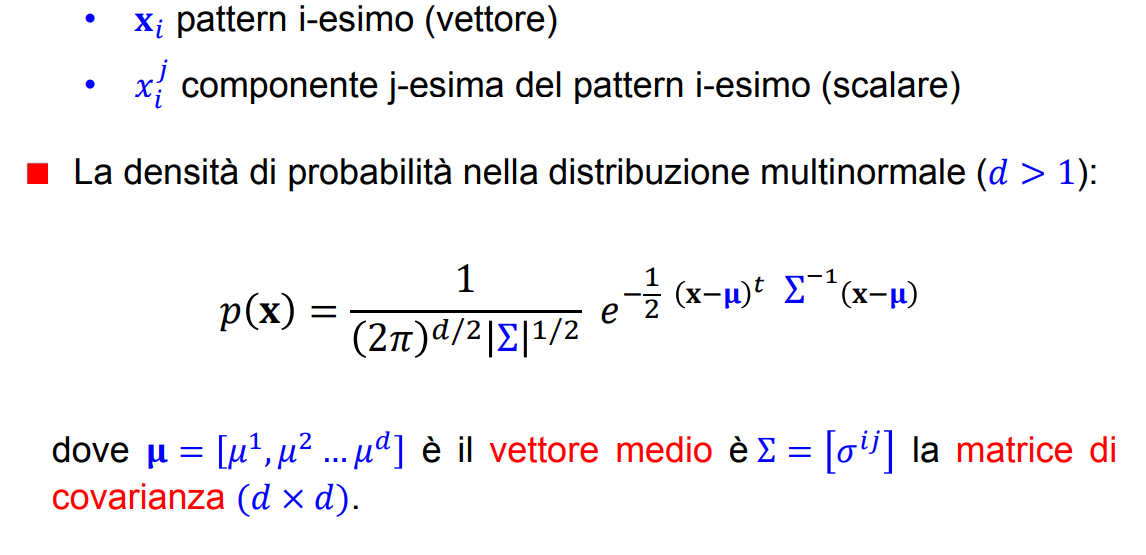
\includegraphics[width=11cm, height=4cm]{Screenshot 2024-12-12 162439.png} % Percorso dell'immagine
    \caption{} % Didascalia per l'immagine
    \label{fig:immagine} % Etichetta per riferimento
\end{figure}
\noindent
$\mu$ è il valor medio (media semplice). $\sigma $ è la deviazione standard, $\sigma^2$ è la varianza.\\\\
La \textbf{Matrice di Covarianza} si indica di solito con $\sum$ ed è la generalizzazione del concetto di varianza al caso di dimensione maggiore di uno. E' una matrice che rappresenta la variazione di ogni variabile rispetto ad altre. E' sempre \textbf{simmetrica} (trasposta uguale) e \textbf{definita positiva}. La \textbf{Matrice Inversa} di una matrice A è pari alla sua Matrice Aggiunta (Trasposta Coniugata) diviso il det(A).\\
\begin{figure}[H] % Usa 'H' per forzare la posizione qui
    \centering % Centra l'immagine
    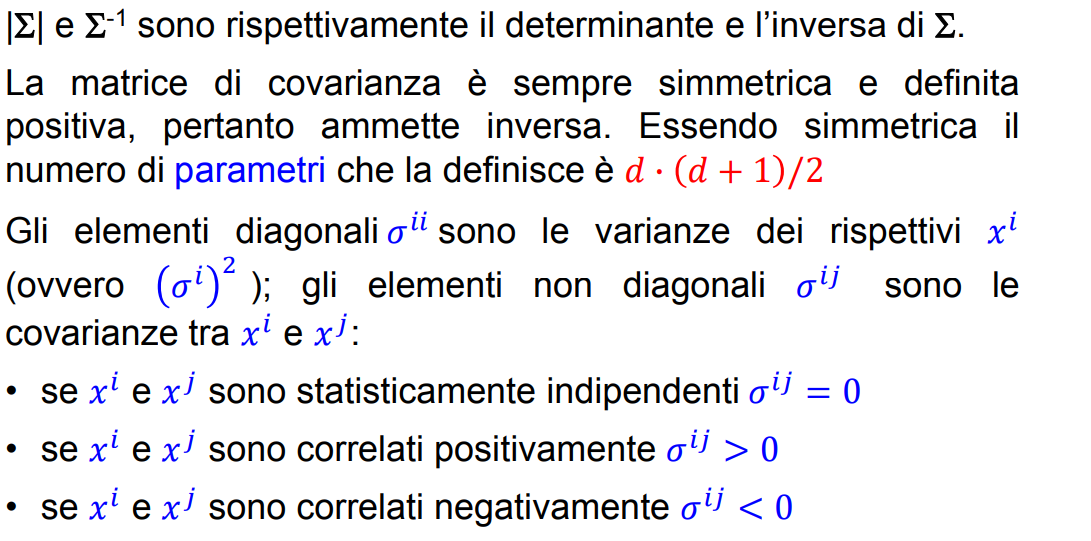
\includegraphics[width=11cm, height=5cm]{Screenshot 2024-12-12 163447.png} % Percorso dell'immagine
    \caption{} % Didascalia per l'immagine
    \label{fig:immagine} % Etichetta per riferimento
\end{figure}
\subsubsection{Distanza Mahalanobis}
La distanza di \textbf{Mahalanobis r} tra \textbf{x} e \textbf{$\mu$} definita dall'equazione:
\begin{figure}[H] % Usa 'H' per forzare la posizione qui
    \centering % Centra l'immagine
    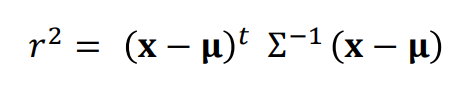
\includegraphics[width=11cm, height=2cm]{immagine_2024-12-12_164824521.png} % Percorso dell'immagine
    \caption{} % Didascalia per l'immagine
    \label{fig:immagine} % Etichetta per riferimento
\end{figure}
\noindent
Definisce i bordi a densità costante in una distribuzione multinormale. Tale distanza viene spesso utilizzata in \textbf{sostituzione della distanza euclidea}, essendo in grado di \textbf{pesare} le diverse componenti tenendo conto dei relativi \textbf{spazi di variazione} e della loro \textbf{correlazione}
\begin{figure}[H] % Usa 'H' per forzare la posizione qui
    \centering % Centra l'immagine
    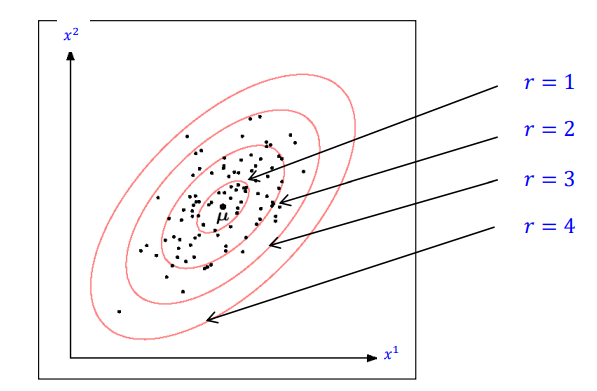
\includegraphics[width=11cm, height=4cm]{Screenshot 2024-12-12 165251.png} % Percorso dell'immagine
    \caption{} % Didascalia per l'immagine
    \label{fig:immagine} % Etichetta per riferimento
\end{figure}
\subsubsection{Esempio con Bayes Parametrico (Multinormali)}
\begin{figure}[H] % Usa 'H' per forzare la posizione qui
    \centering % Centra l'immagine
    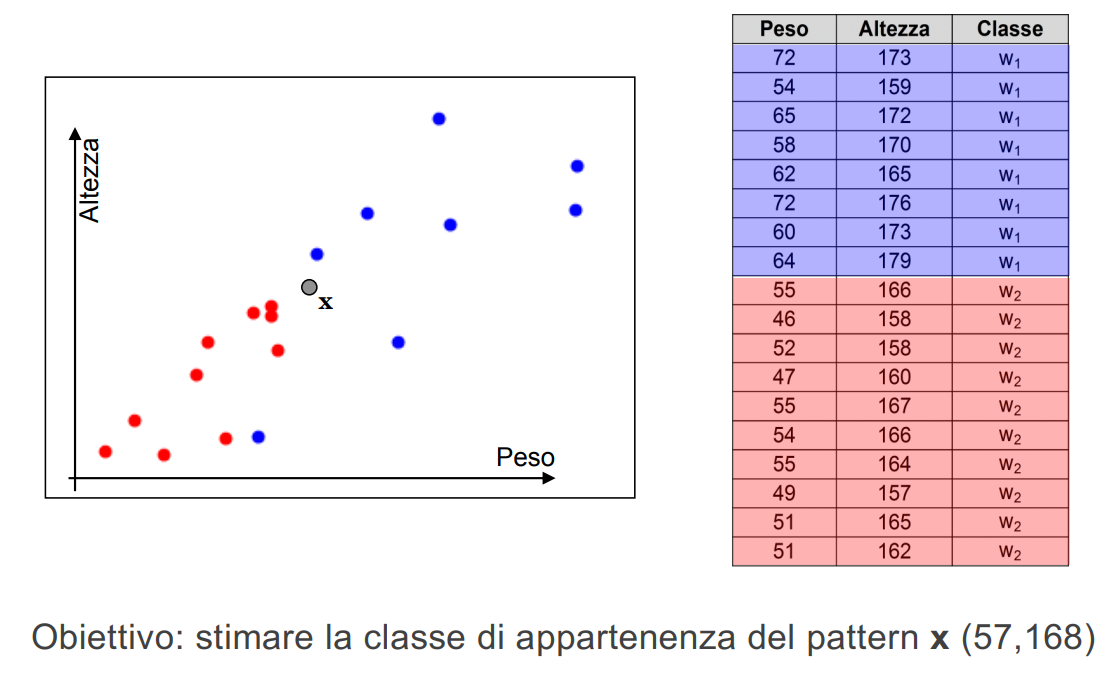
\includegraphics[width=11cm, height=5cm]{Screenshot 2024-12-12 165638.png} % Percorso dell'immagine
    \caption{} % Didascalia per l'immagine
    \label{fig:immagine} % Etichetta per riferimento
\end{figure}
\begin{figure}[H] % Usa 'H' per forzare la posizione qui
    \centering % Centra l'immagine
    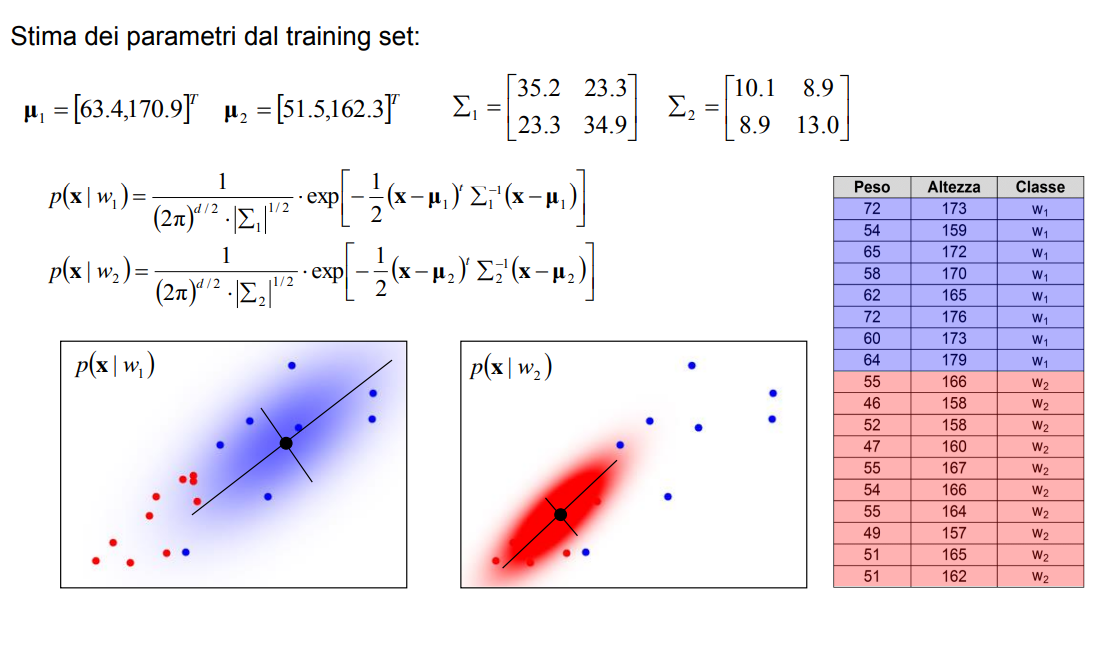
\includegraphics[width=16cm, height=12cm]{Screenshot 2024-12-12 165651.png} % Percorso dell'immagine
    \caption{} % Didascalia per l'immagine
    \label{fig:immagine} % Etichetta per riferimento
\end{figure}
\begin{figure}[H] % Usa 'H' per forzare la posizione qui
    \centering % Centra l'immagine
    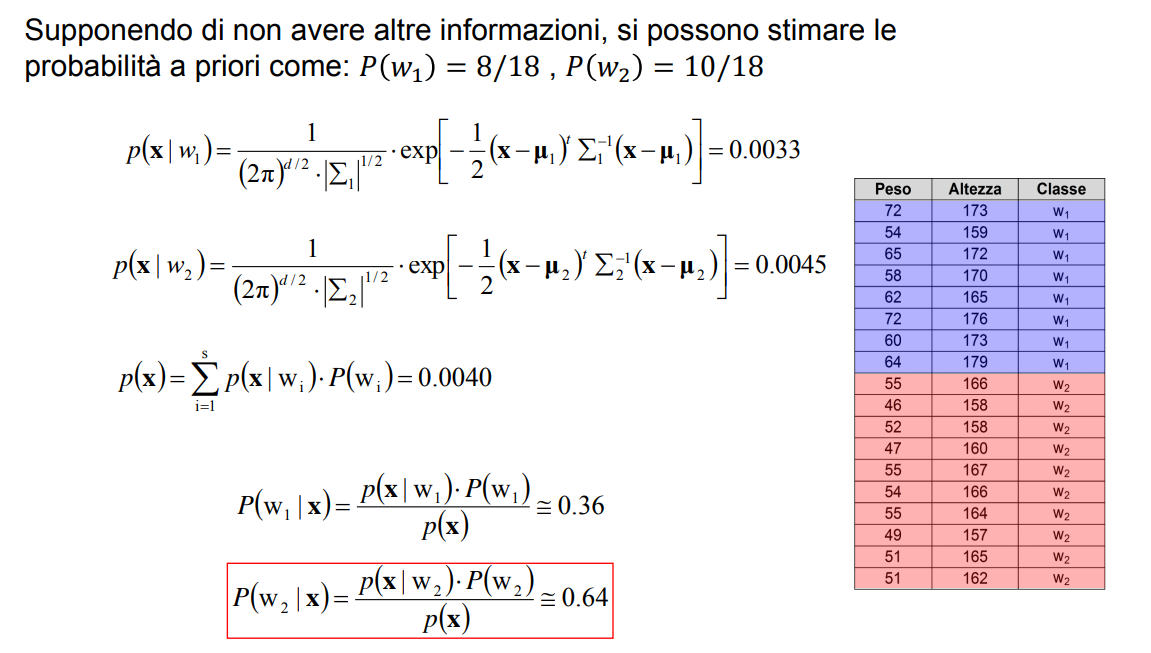
\includegraphics[width=16cm, height=12cm]{Screenshot 2024-12-12 165739.png} % Percorso dell'immagine
    \caption{} % Didascalia per l'immagine
    \label{fig:immagine} % Etichetta per riferimento
\end{figure}
\noindent
Un grande \textbf{vantaggio} del classificatore di Bayes, rispetto ad altri classificatori, è legato al fatto che esso produce un valore di output probabilistico, che può essere utilizzato come confidenza.\\
Infatti, un classificatore può assegnare un pattern x a una classe $w_i$ con diversi livelli di certezza (o confidenza) che possono essere impiegati per: scartare un pattern in applicazioni open-set \textbf{con soglia} costruire un \textbf{multi-classificatore}. Se non serve la confidenza:
\begin{figure}[H] % Usa 'H' per forzare la posizione qui
    \centering % Centra l'immagine
    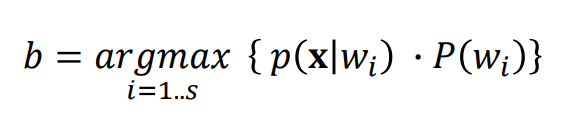
\includegraphics[width=8cm, height=2cm]{Screenshot 2024-12-12 171245.png} % Percorso dell'immagine
    \caption{} % Didascalia per l'immagine
    \label{fig:immagine} % Etichetta per riferimento
\end{figure}
\noindent
Una volta provata una normalità delle distribuzioni, \textbf{si stimano} a partire dei dati, vettore medio $\mu$ e matrice di covarianza $\sum$.\\
Per quanto riguarda le \textbf{probabilità a priori} queste possono essere estratte dalle percentuali di campioni che nel training se appartengono alle diverse classi, o in caso di assenza di informazioni possono essere poste tutte uguali tra loro.\\
Ogni \textbf{nuovo pattern da classificare}, è assegnato a una delle possibili classi in accordo con la regola di Bayes nella quale media e covarianza sono ora note.
\end{document}
